\AtBeginDocument{%
\begingroup\pagestyle{empty}\raggedright\parindent0pt
{\Formular{\Huge{\titulagemfront{}}}}
\vspace{11.25mm}

\LARGE{\autor}
\vfill
\clearpage

%% Créditos ------------------------------------------------------
\raggedright
\linha{copyright}{\copyrightlivro}
\linhalayout{edição brasileira©}{Hedra \ifdef{\ano}{\ano}{\the\year}}
\linha{tradução©}{\copyrighttraducao}
\linha{organização©}{\copyrightorganizacao}
\linha{prefácio©}{\copyrightintroducao}
\linha{ilustração©}{\copyrightilustracao}\smallskip
\linha{título original}{\titulooriginal}
\linha{edição consultada}{\edicaoconsultada}
\linha{primeira edição}{\primeiraedicao}
\linha{agradecimentos}{\agradecimentos}
\linha{indicação}{\indicacao}\smallskip
\linha{edição}{\edicao}
\linha{coedição}{\coedicao}
\linha{assistência editorial}{\assistencia}
\linha{revisão}{\revisao}
\linha{preparação}{\preparacao}
\linha{iconografia}{\iconografia}
\linhalayout{capa e projeto gráfico}{Lucas Kröeff}
%\linha{capa}{\capa}
\linha{imagem da capa}{\imagemcapa}\smallskip
\linha{ISBN}{\ISBN}\smallskip
\begingroup\tiny
\ifdef{\conselho}{\conselho}{\relax}
\par\endgroup\bigskip

\begingroup \tiny

\textit{Grafia atualizada segundo o Acordo Ortográfico da Língua\\
Portuguesa de 1990, em vigor no Brasil desde 2009.}\\


\vfill\textit{Direitos reservados em l\'ingua\\ portuguesa somente para o Brasil}\\\medskip

%
\textsc{editora hedra ltda.}\\
R.~Fradique Coutinho, 1139 (subsolo)\\
05416--011 São Paulo \textsc{sp} Brasil\\
Telefone/Fax +55 11 3097 8304\\\smallskip
editora@hedra.com.br\\
www.hedra.com.br\\
\bigskip
Foi feito o depósito legal.\\\endgroup
\pagebreak\raggedright
%% Front ---------------------------------------------------------
% Titulo
{\Formular{\Huge{\titulagem}}}
\vspace{11.25mm}

{\LARGE{\autor} \par}%\vspace{1.5ex}}
\vspace{6cm} %9.3cm
\ifdef{\organizador}{{\small {\organizador}\\\vspace*{-.5cm} (\textit{organização} e \textit{prefácio})} \par}{}
%\ifdef{\introdutor}{{\small {\introdutor} (\textit{prefácio})} \par}{}
\ifdef{\tradutor}{{\small {\tradutor} (\textit{tradução})}\par}{}\vspace{8.5mm}

{{\footnotesize{} \ifdef{\numeroedicao}{\numeroedicao}{2}ª edição} \par}
%logos
\vfill
\normalsize
\ifdef{\logo}{\IfFileExists{\logo}{\hfill\includegraphics[width=3cm]{\logo}\hfill\logoum{}\\ São Paulo\quad\the\year}}{\logoum\break{} São Paulo\quad\the\year}
%\includegraphics[width=.4\textwidth,trim=0 0 25 0]{logo.jpg}\\\smallskip
\par\clearpage\endgroup
% Resumo -------------------------------------------------------
\begingroup \footnotesize \parindent0pt \parskip 5pt \thispagestyle{empty} \vspace*{-1.7cm}
\baselineskip=.92\baselineskip
\IfFileExists{PRETAS.tex}{\textbf{Fernando António Nogueira Pessoa} (Lisboa, 1888--\textit{id.}, 1935) é o mais
importante poeta português do século~\textsc{xx}. Aos sete anos, muda"-se com a mãe para Durban,
na África do Sul, onde é alfabetizado na língua inglesa.
Em 1905, retorna definitivamente para sua cidade natal e ingressa na Faculdade de Letras
da Universidade de Lisboa. Começa a publicar textos de crítica na revista
\textit{A águia}, em 1912, e a colaborar em jornais e revistas, sendo a principal delas a 
\textit{Orpheu}. Cria os heterônimos Alberto Caeiro, Álvaro
de Campos e Ricardo Reis, o ``semi"-heterônimo'' Bernado Soares e o ortônimo
``Pessoa ele"-mesmo''. Durante sua vida publicou em livro apenas \textit{Mensagem} (1934). 
Trabalhou em Lisboa como tradutor e ``correspondente estrangeiro'' de casas comerciais. 
Falece em decorrência de uma cirrose hepática aos 47 anos, nesta mesma cidade. 

\textbf{Teatro do êxtase} reúne cinco peças de Fernando Pessoa, concebidas 
como poemas dramáticos e destinadas mais à leitura do que à encenação. 
\textit{O~marinheiro} (1915), único drama publicado em vida, foi incluído no
primeiro número da revista \textit{Orpheu} e figura, juntamente com
\textit{Fausto}, como sua peça mais importante.  Definida pelo próprio autor
como um ``drama estático'', a obra de matriz simbolista apresenta o diálogo
entre três mulheres que velam o corpo de uma donzela, sem nenhuma referência
histórica. 
%
\textit{A morte do príncipe} remonta a \textit{Hamlet}, de Shakespeare. 
Trata de um príncipe que
alcança, através de sua viagem delirante pelos arcanos da própria alma,
uma espécie de êxtase visionário, que o leva a afirmar que a única
realidade reside no sonho, isto é, não na própria vida, mas no teatro
da vida. 
%
\textit{Diálogo no jardim do palácio} guarda referências platônicas,
no que diz respeito à reflexão sobre o amor e à dicotomia
entre corpo e alma.
%
\textit{Salomé} insere"-se na rica tradição de leituras do
tema bíblico da \textit{mulher fatal}, ao apresentar o delírio 
da executora de São João Batista diante de sua cabeça decepada. 
%
\textit{Sakyamuni}, por sua vez, representa a ascensão de Siddhartha Gautama ao estado de
iluminação, em que passa a ser reconhecido como Buda. 
%
As peças aqui reunidas são provavelmente as mais acabadas
dentre os muitos fragmentos deixados por seu autor, e apresentam
como eixo comum a concepção pessoana de ``êxtase''.


\textbf{Caio Gagliardi} é professor do Departamento de Letras Clássicas e
Vernáculas da Universidade de São Paulo, na área de Literatura
Portuguesa; mestre e doutor em Teoria e História Literária pela \textsc{Unicamp}
e pós"-doutor em Teoria Literária pela \textsc{usp}. É também pesquisador da obra
de Fernando Pessoa e editor do site \textit{Crítica \& Companhia}.



}{% 
\ifdef{\resumo}{\resumo\par}{}
\ifdef{\sobreobra}{\sobreobra}{}
\ifdef{\sobreautor}{\mbox{}\vspace{4pt}\newline\sobreautor}{}
\ifdef{\sobretradutor}{\newline\sobretradutor}{\relax}
\ifdef{\sobreorganizador}{\vspace{4pt}\newline\sobreorganizador}{\relax}\par}
\thispagestyle{empty} \endgroup
\ifdefvoid{\sobreautor}{}{\pagebreak\ifodd\thepage\paginabranca\fi}
% Sumário -------------------------------------------------------

\sumario{}
%\IfFileExists{INTRO.tex}{\chapter[Introdução, por Caio Gagliardi]{Introdução}
\hedramarkboth{Introdução}{Caio Gagliardi}

\textsc{Fernando Pessoa} planejou uma grande obra teatral, antes concebida para
ser lida do que encenada. Embora tenha escrito mais de trinta peças em
português e em inglês, em prosa e em verso, a sua quase totalidade foi
deixada inacabada e desconhecida do grande público. Em algumas
anotações do autor a respeito dessa fração menos conhecida de sua obra,
encontramos registrada a expressão “Teatro d’êxtase”, que emprestamos a
esta edição. 

Não há uma listagem completa das peças que comporiam esse conjunto, mas é certo
que a palavra “êxtase” identifica uma característica comum às que aqui
estão reunidas: nelas, há sempre um momento em que as personagens
parecem encarnar a figura do sonhador visionário, que viaja, através de
conjecturas, para além do real imediato, deixando-se absorver por um
estado de consciência independente de toda e qualquer ação externa. O
substantivo “êxtase” (do grego \textit{ekstasis}) refere-se a um estado
da alma absorta na contemplação de Deus e do mundo sobrenatural,
definição que condiz, de modo mais ou menos direto, com os enredos das
peças, em que há sempre uma forma de intuição ou vidência que é
atribuída a uma de suas personagens. Ainda do ponto de vista
psicanalítico -- que não era estranho a Pessoa --, “êxtase” é um estado
nervoso caracterizado pela perda da consciência da própria existência,
o que sintetiza bem, como veremos mais adiante, um dos momentos de
\textit{O marinheiro}, a principal peça que integra este conjunto.

\section{\mbox{Das peças que integram esta edição}}

\textit{O marinheiro} foi a única peça publicada em vida por Pessoa. Foi
com ela, aliás, que seu autor, até então mais conhecido pelo leitor
português como polemista e crítico literário, estreou no primeiro
número da revista \textit{Orpheu}, a publicação mais importante do
modernismo em Portugal. Segundo Pessoa, a peça teve uma primeira versão em 1913
(conforme a data que acrescenta ao seu final), e foi revisada até a sua
publicação, em 1915. Além disso, \textit{O marinheiro} antecipa com
especial habilidade artística aspectos marcantes da poética pessoana,
dentre os quais o processo de despersonalização dramática, da qual
resulta a heteronímia. Devido à sua importância central para o conjunto
da obra de Fernando Pessoa -- embora não fosse demasiado afirmar, para a
história do teatro em língua portuguesa --, optamos por dedicar-lhe um
estudo exclusivo. 
\renewcommand{\caption}[1]{{\small\textit{#1}}}
\begin{figure}
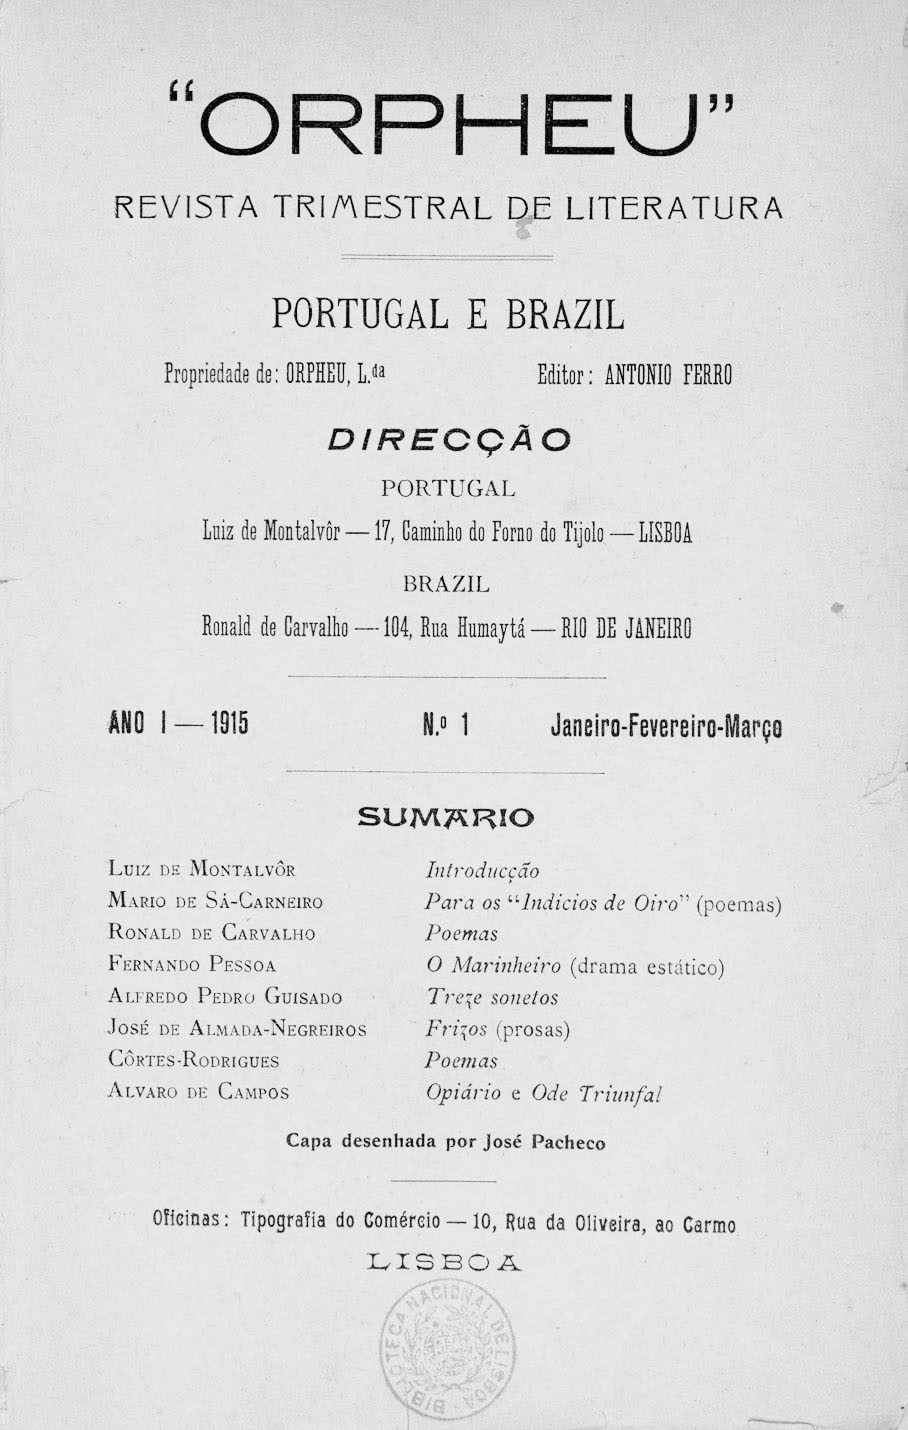
\includegraphics[width=\textwidth]{3.png}
\caption{Frontspício do n.~1 da revista \emph{Orpheu}}
\end{figure}

Além de \textit{O marinheiro}, reúnem-se aqui outros quatro dramas,
\textit{A morte do príncipe}, \textit{Diálogo no jardim do
palácio}, \textit{Salomé} e \textit{Sakyamuni}.\footnote{ Esses textos
são, na sua origem, manuscritos e fragmentos datilografados encontrados em folhas dispersas,
incluindo alguns exemplares da revista \textit{A águia}. 
Muitas dessas páginas não foram identificadas pelo autor, e, à margem do texto, 
Pessoa deixou anotadas variantes para muitos termos que empregou, o que revela seu estágio ainda
inacabado.
Todo esse material foi transcrito, coligido e ordenado pela
crítica portuguesa Teresa Rita Lopes, sem a qual a expressão “o teatro
de Pessoa” teria uma dimensão bem mais restrita do que a atual. Com
exceção ao \textit{Fausto}, texto escrito durante toda a vida literária
de seu autor, as peças aqui publicadas são aquelas que apresentam
melhor acabamento formal.}

\textit{A morte do príncipe} recebeu encenações em Portugal e na
Argentina, e foi adaptada para o cinema em 1991, com o mesmo título e
sob direção de Maria de Medeiros. Trata-se de um texto praticamente
acabado, que remete aos monólogos de \textit{Hamlet}, de Shakespeare,
mas com fortes ecos de Mallarmé: “Todo este universo é um livro em que
cada um de nós é uma frase”. Difícil não projetar sobre a personagem
“X” a figura de Horácio, fiel amigo de Hamlet. O tom de certas
passagens de teor metalinguístico é o mesmo atingido por trechos
análogos do \textit{Livro do desassossego}. A exemplo das demais
personagens das peças aqui reunidas, o príncipe alcança, através de sua
viagem delirante pelos arcanos da própria alma, uma espécie de êxtase
visionário, de crise perceptiva, que o leva a afirmar que a única
realidade reside no sonho, isto é, não na própria vida, mas no teatro
da vida: “As princesas que eu sonhei é que existem\ldots{} As da terra são
apenas as bonecas com que as outras brincam, vestindo-as, corpo e alma,
a seu modo\ldots{}”
Entre os fragmentos que foram reunidos para recompor a peça, duas páginas foram
datilografadas no verso de um panfleto em defesa de Raul Leal, atacado por uma organização 
de estudantes, ``Sobre um Manifesto de Estudantes'', escrito em 
abril de 1923. Além disso, Teresa Rita Lopes transcreveu uma folha datilografada
que traz a data de 05--10--1932.
Embora dialogada, toda a cena se passa como se fosse um
monólogo.

\textit{Diálogo no jardim do palácio} é também uma peça aparentemente
concluída, que guarda fortes ecos dos diálogos platônicos,
especificamente no que tange a reflexão sobre o amor e a dicotomia
entre corpo e alma. Como acontece com as demais peças aqui publicadas,
este diálogo entre duas personagens, apenas indicadas por A e B, é um
interlúdio temporal, uma espécie de suspensão cronológica em que o eu
se observa cindido em dois, refletindo sobre a tópica do \textit{amabam
amare} (amar o amor), de Santo Agostinho, e antecipando a reflexão mais
sistemática que Pessoa realizaria no âmbito “sensacionista”: 
\begin{hedraquote}
Há grandes interiores de continentes dentro de nós, com mistérios a
desvendar. Quem sabe, amor, se raças diferentes das nossas habitarão
esses sítios desconhecidos (inexplorados)? Habituei-me sempre a olhar
para as minhas sensações como para uma coisa exterior.
\end{hedraquote}

Parte do texto
foi escrita à mão em algumas páginas de um dos números da revista
\textit{A águia}, de 1913. Este diálogo foi representado em conjunto
com as outras peças aqui mencionadas, em Portugal e no Brasil.
\begin{figure}
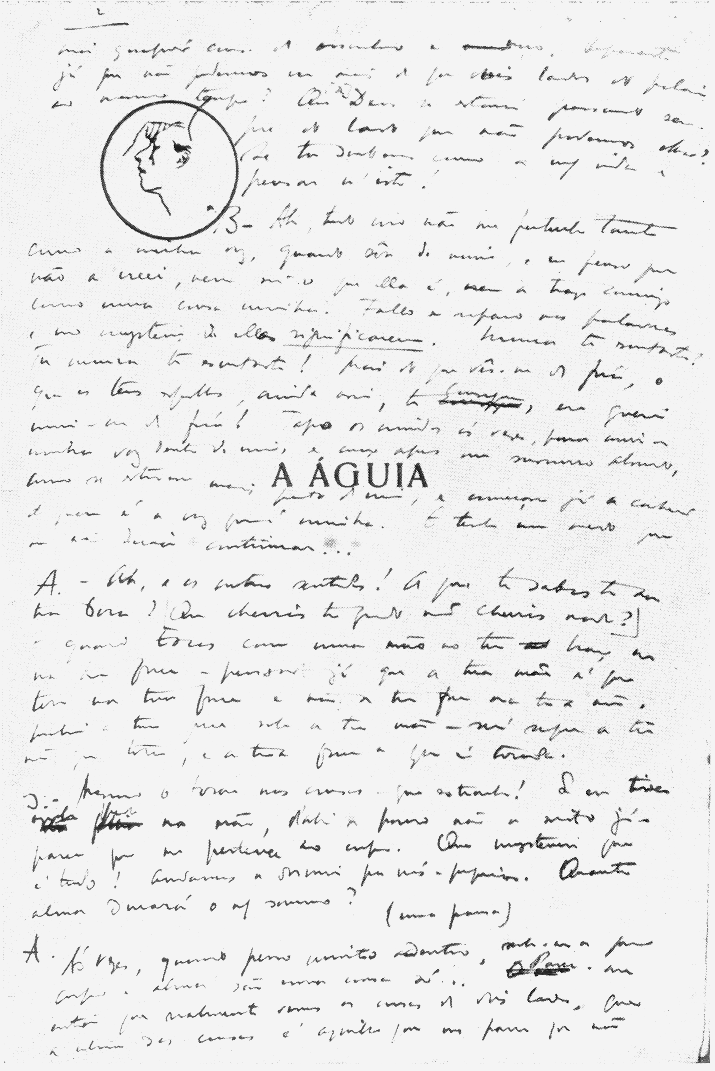
\includegraphics[width=\textwidth]{4.png}
\caption{Manuscrito feito sobre a edição da revista \emph{A águia}}
\end{figure}

Com \textit{Salomé}, Pessoa insere-se na rica tradição de releituras do
tema bíblico da \textit{mulher fatal}, que povoa o imaginário cultural
dos finais do século \textsc{xix}. Apontada como executora de João Batista, no
\textit{Novo Testamento}, Salomé foi retratada na pintura de Moreau, na
ópera de Strauss e na literatura de autores como Flaubert, Mallarmé,
Wilde, Huysmans e Laforgue. A peça que Fernando Pessoa nos legou, e na
qual alcança inaudita suspensão onírica, é uma das menos conhecidas
entre as releituras que o mito bíblico inspirou. Embora fragmentada, a
\textit{Salomé} de Pessoa já ganhou os palcos, além de ter se
transformado em ópera de câmara em seu país de
origem. Uma das páginas desse drama foi manuscrita no verso de uma carta
datada de 9 de março de 1914.

Finalmente, \textit{Sakyamuni} é uma
espécie de encenação budista que pertenceria a um conjunto de três
peças, das quais conhecemos somente um outro título, \textit{Calvário},
esta centrada na figura de Cristo. \textit{Sakyamuni} retoma o processo
de ascensão do príncipe do Himalaia, Siddhartha Gautama (566--468 a.C.),
a Sakyamuni, ou seja, o sábio do clã Shakya, e posteriormente sua
iluminação, a partir da qual passou a ser chamado de Buda. O termo
\textit{Boddhisattva} era usado pelo Buda para se referir a si mesmo em
todo o período anterior à sua iluminação, incluindo suas vidas
anteriores. “Buda” foi, inclusive, um título cogitado por Pessoa para
esse drama. Sem indicação de data, a peça nos sugere interessante clave de leitura para o
vertiginoso processo de despersonalização poética em que resultou a
heteronímia: “Tornado a Diversidade Absoluta, o Abismo Puro, morrerás
de ti próprio. E tudo será o Nirvana atingido, e o Fim [dourado] da
Estrada''.


\section{O espaço primordial do drama em \textls{O marinheiro}}

Pessoa definiu \textit{O marinheiro} como um
\textit{drama estático}. A expressão, em voga entre
autores franceses do fim do século \textsc{xix}, revela
a existência de uma forte identidade entre sua peça e o teatro
simbolista dos anos 1890, no qual, amiúde, os diálogos 
não são senão intervalos que preparam o leitor para 
as pausas e os longos silêncios,
e em que a encenação apresenta forte apelo simbólico.
Assim como sucedeu com o romance, o teatro simbolista 
foi responsável por superar
as convenções naturalistas de representação. Não se tratava, ao
contrário do que se pode pensar, de uma experiência 
de ruptura, pura e simplesmente; o ``\textit{théatre statique}'',
tal como referido por seus epígonos
de língua francesa, antes de designar um gênero, teria sido uma
qualidade própria das grandes peças da Antiguidade Clássica. Para o
principal nome do teatro desse período, 
o belga Maurice Maeterlinck, a
maior parte das tragédias de Ésquilo são 
``\textit{tragédies immobiles}''. Mas o
protótipo desse tipo de drama é 
\textit{Hamlet}, de Shakespeare. A seu
respeito, não é impreciso afirmar que os 
monólogos interiores de seu
protagonista provocaram verdadeiro fascínio no imaginário
simbolista.\footnote{ M. Maeterlinck.
\textit{Le Trésor des Humbles}.
Apud Teresa Rita Lopes. \textit{Fernando Pessoa 
et le drame simboliste: héritage et création}.
Lisboa, Paris, Foudation Calouste Gulbenkian:
Centre Culturel Portugais, 1985, p.~17.} Em síntese, o drama
simbolista conferiu à \textit{imobilidade} o status
de valor próprio das grandes peças. 

Segundo Robert Bréchon, com o seu drama \textit{Os cegos} (1890),
Maeterlinck forneceu a \textit{O marinheiro} seu 
“modelo formal da ação dramática”.\footnote{ Robert Bréchon.
\textit{Estranho estrangeiro}.
Rio de Janeiro: Record, 2000. pp.~176--7.} 
Teresa Rita Lopes, autora do
mais importante trabalho sobre a relação de Pessoa com o drama
simbolista, revela que a biblioteca do poeta, hoje 
hospedada na Casa Fernando Pessoa, em Lisboa, 
contém a mais conhecida peça de Maeterlinck,
\textit{Les Aveugles}, profusamente anotada. Para
a pesquisadora, a identificação de influências não deve sugerir,
contudo, uma relação de dívida com o teatro simbolista, uma vez que
\textit{O marinheiro} supera, enquanto realização formal e 
em densidade psicológica, seus modelos imediatos.

Outra característica que o drama simbolista emprestou a \textit{O
marinheiro} é a sublevação das personagens com relação às suas
falas. Em outras palavras, no drama simbolista as personagens 
parecem sempre menos importantes do que as palavras que enunciam. 
Elas, por vezes, chegam mesmo a se espantar com o que dizem. 
Esse traço é marcante em autores como Mallarmé e Hofmannsthal, 
que, nas palavras de Anna Balakian, cultivaram o “poder mágico 
da palavra”.\footnote{ Anna Balakian.
\textit{O simbolismo}. São Paulo: 
Perspectiva, 1985, p.~109.} O que talvez seja axial 
nessa concepção de teatro é sua aproximação com a
poesia, gênero em que as palavras apresentam especial densidade.
Algumas peças de Yeats, por exemplo, são derivações de seus 
poemas, o que é um dado representativo da ausência de 
fronteiras bem demarcadas entre os gêneros.
Afinal, tratava"-se já de um teatro lírico de ruptura
com as convenções do drama, cujo tom sepulcral delegava
à morte seu papel simbólico central. 

Num manuscrito, provavelmente de 1914, Pessoa formula
essa sua concepção de teatro:

\begin{hedraquote}
Chamo teatro estático àquele cujo enredo 
dramático não constitui ação --
isto é, onde as figuras não só não
agem, porque nem se deslocam nem
dialogam sobre deslocarem"-se, mas
nem sequer têm sentidos capazes de
produzir uma ação; onde não há conflito
nem perfeito enredo. Dir"-se"-á
que isto não é teatro. Creio que o é
porque creio que o teatro tende a
teatro meramente lírico e que o enredo
do teatro é, não a ação nem a
progressão e consequência da ação --
mas, mais abrangentemente, a
revelação das almas através das 
palavras trocadas e a criação de
situações [\ldots{}]. Pode haver revelação
de almas sem ação, e pode haver
criação de situações de inércia, momentos 
de alma sem janelas ou portas
para a realidade.\footnote{ Fernando Pessoa. \textit{Páginas de estética e de teoria e crítica
literárias}. 2ª. ed., org.~de Georg Rudolf Lind e Jacinto do Prado
Coelho. Lisboa: Ática, 1973, p.~112.}
\end{hedraquote}

O quarto, onde transcorre \textit{O marinheiro}, tem o formato circular, a exemplo do palco grego,
cujo centro, destinado ao plano terrestre da representação,
é também esférico. No centro do quarto, por sua vez, no alto
de uma mesa, há um caixão onde jaz uma donzela de branco.
Não sabemos quem ela foi, que relação teve
com suas veladoras, tampouco quando e em que lugar se situa esse
castelo. A indicação isolada de que ele
é \textit{antigo} se apresenta
como indício de uma ancestralidade mítica, isto é, de que a cena se
passe fora do tempo histórico. Estamos diante de um 
drama imemorial,
portanto, cujo prenúncio já se revela em sua primeira 
fala, “Ainda não
deu hora nenhuma”, e perpassa todo o texto, “Quem sabe se nós
poderíamos falar assim se soubéssemos a hora que é?”.
A vigília das três
donzelas -- não por acaso identificadas como “veladoras” --
assume já um caráter alegórico no drama, por atuar como 
metáfora da existência. Daí
a ancestralidade que é própria, afinal, do
\textit{leitmotiv}, do seu motivo condutor:
a morte ocupa o centro do quarto e do drama, e as
veladoras, à sua volta, como Sherazade para escapar a ela,
conversam,
contam histórias, suspendendo a \textit{physis},
a realidade ou seu fim natural. 
Exemplar é, por isso, a fala da segunda veladora: “Contemos
contos umas às outras\ldots{} Eu não sei contos nenhuns, 
mas isso não faz mal\ldots{} Só viver é que faz mal\ldots{}”. 
``Navegar é preciso, viver não é
preciso'', afirmará Pessoa mais tarde. Eis um dos 
frutos semeados por \textit{O marinheiro} em sua poética.

Curiosamente, esse caráter \textit{mítico} da peça não impede, ao
contrário do que se poderá supor, que ela respeite a lição 
aristotélica da unidade de espaço e de tempo: 
o drama pessoano apresenta tanto
duração definida -- transcorre no período de
uma madrugada -- quanto, como se disse, espaço
demarcado -- a torre de um castelo. Além disso,
chama a atenção o fato de a tragédia antiga 
nunca apresentar mais do
que três personagens contracenando, exatamente 
o número de donzelas em
\textit{O marinheiro}. Os tragediógrafos antigos 
observavam a regra de
não falar uma quarta personagem numa mesma cena, conforme vem
registrado no preceito de Horácio, na epístola aos Pisões,
``\textit{nec quarta loqui persona laboret}'' literalmente 
``e uma quarta personagem não se empenhe em
falar''.\footnote{ Horácio. \textit{Arte poética}. Ed.
bilíngue. Trad.  R. M. Rosado Fernandes. Lisboa: Clássica, s.~d.
v.~193.} No \textit{Agamêmnon},
de Sêneca, por exemplo, no último ato,
Cassandra, embora o tempo todo presente em cena, junto com
Clitemnestra, Egisto e Electra, só fala depois que esta última se
retira, levada para o exílio.\footnote{ Sêneca,
\textit{Agamêmnon}.
Intro., trad. e org. de José Eduardo Lohner.
São Paulo: Globo,
2009.} Em \textit{O marinheiro}, a quarta personagem está morta. 

Ao que parece, existe nesse drama um jogo de definições e
indefinições que não pode ser desprezado.

Embora tenha sido produzido em prosa, \textit{O marinheiro} é 
permeado
de um lirismo sugestivo, cinzelado por pausas e reticências.
Associado
a ele, a sensação de irrealidade acompanha sua leitura, como se uma
leve bruma encobrisse a cena única, toldando"-a com uma atmosfera de
sonho, própria da sondagem psicológica presente nos diálogos. Essa
atmosfera carrega também algo de sinistro. Isso porque a 
condução do
drama é análoga à de um suspense metafísico: em mais de um momento das
falas das personagens, algo parece estar para ser revelado, e a
previsão dessa descoberta causa"-lhes espanto e temor. 

Vem a propósito desse comentário um importante trecho escrito em inglês
por Pessoa, traduzido pelo crítico José Augusto Seabra, no qual o
escritor sublinha o caráter trágico da peça e revela seu juízo
especialmente positivo sobre o desenlace:

\begin{hedraquote}
Começando de uma forma muito simples, o drama evolui 
gradualmente para
um cume terrível de terror e de dúvida, 
até que estes absorvem em si as
três almas que falam e a atmosfera da 
sala e a verdadeira potência do
dia que está para nascer. O fim da peça 
contém o mais sutil terror
intelectual jamais visto. Uma cortina de 
chumbo tomba quando elas não
têm mais nada a dizer uma às outras nem mais nenhuma razão para
falar.\footnote{ Apud José Augusto Seabra.
\textit{Fernando Pessoa ou
o poetodrama}. São Paulo: Perspectiva, 1974, p.~31. O trecho vem
reproduzido no original segundo a edição da \textit{Obra poética} 
da Nova Aguilar.}
\end{hedraquote}

A ausência de demarcação do tempo histórico
da cena está associada à
sensação de irrealidade que ela produz em seu leitor e nas próprias
personagens. Estas, por seu turno, não compõem 
um conflito; ao invés de
agirem, apenas conversam, e seus diálogos são 
prolíficos em conjecturas
existenciais. As falas das veladoras, a certa 
altura da peça, deixam de
demarcar espaços de enunciação distintos ou de identificar as
personagens, para confundi"-las umas com as outras. Ganha força a
sensação no leitor de que essas vozes não se prendem a um corpo
definido. À medida que a leitura avança, as veladoras se evanescem,
desmaterializam"-se enquanto personagens, e as falas, 
já incorpóreas, e
sem referência no espaço e no tempo, deixam transparecer o tom
monocórdio do texto. O diálogo se enfraquece a ponto de 
se remodular em
uníssono, e as três vozes convergem, finalmente, 
num monólogo. A partir
de então, a leitura já não é a de um drama que se 
passa na torre de um
castelo, mas dentro da mente humana. Das veladoras, embora ainda
identificadas como enunciadoras, resta apenas o espectro, e a peça,
como que nos convidando à releitura, permite entrever sua imagem
latente: de uma única personagem em conversa consigo mesma. Eis o
espaço primordial desse drama.

\paragraph{Uma \textit{plaquette} ou o mais alto grau do sonho}

Em 1915, Fernando Pessoa já havia escrito alguns dos 
seus principais
poemas, incluindo parte importante da poesia 
heteronímica. Dentre um
conjunto notável de textos, Pessoa escolhe
\textit{O marinheiro} para
figurar como seu primeiro texto publicado na
\textit{Orpheu}, a revista
que inaugura o modernismo em Portugal,
e certamente a mais genuinamente
pessoana delas. A \textit{Orpheu} veicula 
também, mais adiante, dois
textos antológicos de Álvaro de Campos, a
“Ode triunfal” e “Opiário”,
embora estes poemas não façam parte de um plano
original de publicação,
tendo sido incluídos na revista sob a justificativa de preencher
espaço. O fato de o autor de \textit{O marinheiro}
tê"-lo escolhido,
depois de submetê"-lo a profunda reelaboração,
para compor o primeiro
número da revista \textit{Orpheu}, dá mostras, afinal, do especial
apreço que nutria por seu “drama estático”.
A julgar pelo frontispício
da revista, que traz o desenho de José Pacheco,
de uma jovem nua sobre
um fundo azul e entre duas grandes velas 
(uma veladora?), não é difícil
imaginar o valor que a peça de Pessoa teve
para os leitores da \textit{Orpheu}
e, por extensão, para o modernismo português de modo geral. 

Sua leitura, não por acaso, permite a fácil
identificação de alguns dos
temas mais caros à poesia de Pessoa: as dúvidas existenciais; a
intuição de que a vida é sonho; o desdobramento
da voz; a clivagem do
eu num espaço aberto entre aquele que sente e aquele
que pensa, ou entre
aquele que pensa e que diz; o fado da autoconsciência; 
o adiamento pelo sono. 

Embora seja um drama, e como tal já tenha
ocupado palcos em diferentes
países, todas as encenações de \textit{O marinheiro}
ocorreram após a morte de seu autor.
Na verdade, seu texto não foi escrito para ser
encenado, tanto é que Pessoa procurou 
publicá"-lo em revista,
sem cogitar a montagem, considerando"-o como um “poema dramático”.  
\begin{figure}
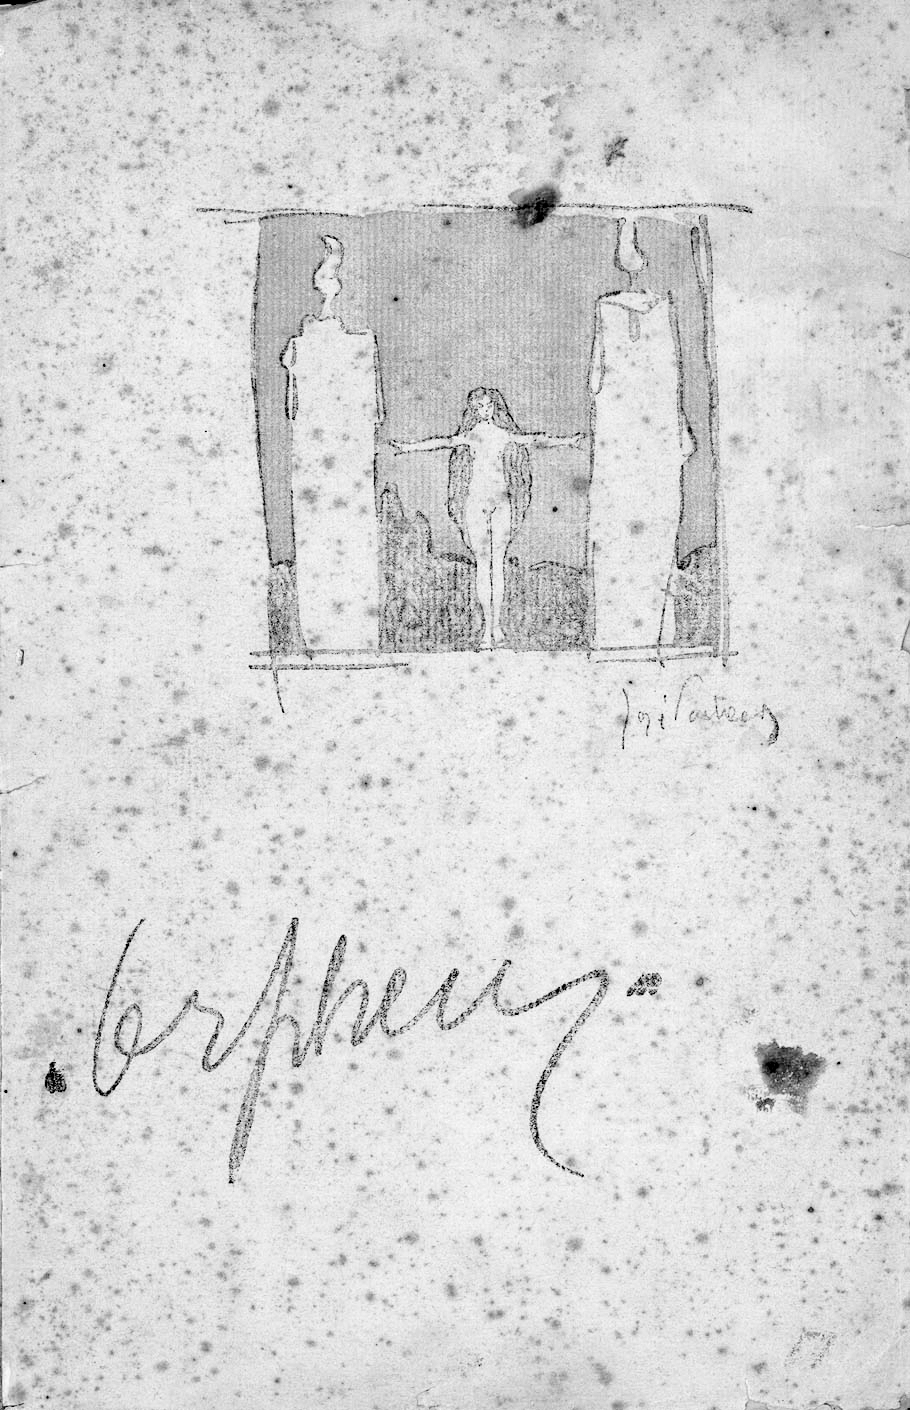
\includegraphics[width=\textwidth]{2.png}
\caption{Desenho reproduzido na capa da revista \emph{Orpheu}, n.~1.}
\end{figure}

Pessoa diz tê"-lo escrito na noite de 11
para 12 de setembro de 1913. Mas o texto 
foi publicado pela primeira vez dois anos
depois, na
\textit{Orpheu}, n. 1 (Lisboa, 1915).
A esse respeito, o autor observa ainda, 
numa carta enviada ao poeta e companheiro de geração Armando
Côrtes"-Rodrigues, que, entre a data da escrita e a
da publicação de seu
drama, submeteu"-o a uma profunda revisão,
deixando"-o bastante diferente
do que era em sua versão original; em suas palavras:

\begin{hedraquote}
O meu drama estático “O marinheiro” está bastante alterado e
aperfeiçoado; a forma que v. conhece é apenas a primeira e
rudimentar.
O final, especialmente, está muito melhor.
Não ficou, talvez, uma coisa
\textit{grande}, como eu entendo as coisas grandes;
mas não é coisa de
que me envergonhe, nem -- creio -- me
venha a envergonhar.\footnote{
Carta a Armando Côrtes"-Rodrigues, 4 de março de 1915.
\textit{In}: \textit{Fernando Pessoa --
Correspondência 1905--1922}. Org.~de Manuela Parreira
da Silva. São Paulo: Companhia das Letras, 1999, p.~159.}
\end{hedraquote}

Aquilo que motivou tal revisão, e que é, portanto, determinante na
composição do texto de que dispomos, foi o fato de Álvaro Pinto,
diretor da revista \mbox{\textit{A águia}}, ter se recusado a publicar
\textit{O marinheiro}, em 1914, numa \textit{plaquette},
ou seja, num
pequeno folheto encadernado. Após esta rejeição 
e a decorrente revisão
do texto, a peça sairia não mais numa publicação de teor
saudosista,
mas no número de estreia da mais importante
revista modernista de seu
país, o que faz pensar no quão decisiva deve 
ter sido essa recusa na depuração da peça. 

A bem dizer, a recusa de Álvaro Pinto em publicar a peça numa
\textit{plaquette} do grupo da \textit{Renascença}
\textit{Portuguesa},
do qual \textit{A águia} era o órgão principal, 
foi o último episódio
relevante de um afastamento progressivo do
poeta com relação ao grupo
saudosista. A ruptura tardaria até o 
fim daquele ano para acontecer,
mas se observarmos com atenção, já o seu
texto anterior publicado na
revista, “Na floresta do alheamento”, 
sai com atraso de um número, o
que se documenta em carta de Pessoa
a seu editor nos seguintes termos:
“O ‘Na floresta do alheamento’ será ultraexcessivo, em matéria de
requinte, para que achem prudente que \textit{A águia} o insira?
Diga"-mo francamente.”\footnote{ Carta a Álvaro Pinto,
Lisboa, 29 de julho de 1913. \textit{In}: Fernando Pessoa --
\textit{Correspondência}
1905--1922. Op.~cit., 1999, p.~100.} 

Esse texto, que é um dos primeiros fragmentos do \textit{Livro do
desassossego}, naquele momento assinado 
com o próprio nome do poeta
(não existia, ainda, Bernardo Soares), apresenta uma atmosfera
decadente, tematiza o tédio e a inquietude existencial,
e representa
muito pouco o projeto \textit{renascente}.
Pessoa procurava desfiar, a
partir de uma sensação sua, a realidade interior, convertendo"-a,
através de imagens complexas, numa paisagem exterior.
Embora ainda com
ares decadentes, nesse momento se delineia pela obra de Pessoa uma
concepção que permanecerá muito sólida, e que o acompanhará até os
últimos poemas: “Quem quisesse resumir numa palavra a
característica
principal da arte moderna encontra"-la"-ia, 
perfeitamente, na palavra
\textit{sonho}. A arte moderna é arte de 
sonho.”\footnote{ O manuscrito
em que Pessoa faz essa afirmação é, segundo
os organizadores do volume,
provavelmente de 1913, o mesmo ano de escrita 
de \textit{O marinheiro}. Em
Fernando Pessoa. \textit{Páginas
de estética e de teoria e crítica
literárias}, op.~cit., p.~153.} 

Esse novo modo de encarar a arte,
que se afirma reiteradamente tanto na
prosa teórica de Pessoa quanto na do
\textit{Livro do desassossego}
(“Sonhar é encontrarmo"-nos. Vais ser o Colombo da
tua alma.”\footnote{ Bernardo Soares. 
\textit{Livro do desassossego}, org., intro. e notas
de Richard Zenith. São Paulo:
Companhia das Letras, 2006, p.~440.}),
despertava no próprio poeta a consciência
do quão distante ele já se
encontrava das diretrizes saudosistas.
Por esse motivo, quando Pessoa
antecipa a Álvaro Pinto o envio próximo de
\textit{O marinheiro}, já
tem, se observarmos com atenção, plena
consciência de que a peça não
poderia sair em \textit{A águia}: 

\begin{hedraquote}
Dentro em pouco, mandar"-lhe"-ei, para a \textit{Renascença}, caso queira
editar, um escrito meu -- uma peça em um ato, dum gênero especial a que
eu chamo \textit{estático}. Claro está que o meu amigo com toda a
franqueza me dirá, depois de ler a peça, se convém realmente editá"-la.
Exijo, e não me ofenderei com uma recusa -- uma franqueza absoluta.

A peça formará uma mera \textit{plaquette}. Não lha remeto para
\textit{A águia} porque para esse fim é, além de extensa, vagamente
imprópria.\footnote{ Carta a Álvaro Pinto,
Lisboa, 25 de maio de 1914.
Op.~cit., p.~116.}
\end{hedraquote}

Ao julgar que sua peça é imprópria para o órgão saudosista, Pessoa se
mostra ciente de que seu novo escrito anuncia caminhos inauditos não
apenas para o conjunto de sua obra, como para a literatura de seu país.
O que parece estar no gérmen dessa descoberta é a concepção de que a
tão obstinadamente perseguida “nova literatura” encerra a investigação
da própria alma do criador. É ainda em “Na floresta do alheamento” que
esse novo caminho vem anunciado, pouco depois
concretizado em \textit{O marinheiro}:

\begin{hedraquote}
O mais alto grau do sonho é quando, criado um quadro com personagens,
vivemos \textit{todas elas} ao mesmo tempo -- \textit{somos todas essas
almas conjunta e interativamente}. É incrível o grau de
despersonalização e encinzamento do espírito a que isto leva e é
difícil, confesso"-o, fugir a um cansaço geral de todo o ser ao
fazê"-lo\ldots{} Mas o triunfo é tal!\footnote{ Bernardo Soares. 
\textit{Livro do desassossego}. Op.~cit., p.~444.} 
\end{hedraquote}

Pessoa passaria então a levar às últimas consequências a concepção de
que a única realidade para si é ele próprio, e a investigar as leis de
sua personalidade através da tomada de consciência dos processos
mentais através dos quais se dão o conhecimento, as emoções e as
sensações, e, sobretudo, a refletir sobre como eles são convertidos em
arte. A literatura irá adquirir tal importância nesse processo, que
Pessoa assumirá que não sente, senão literariamente, que é poeta em
período integral, e que, portanto, o eu individual não está em lugar
algum: ele é muitos e nenhum ao mesmo tempo: 

\begin{hedraquote}
Tornei"-me uma figura de livro, uma vida lida. O que sinto é (sem que eu
queira) sentido para se escrever que se sentiu. O que penso está logo
em palavras, misturado com imagens que o desfazem, aberto em ritmos que
são outra coisa qualquer. De tanto recompor"-me destruí"-me. De tanto
pensar"-me, sou já meus pensamentos mas não eu. Sondei"-me e deixei cair
a sonda; vivo a pensar se sou fundo ou não, sem outra sonda agora senão
o olhar que me mostra, claro a negro no espelho do poço alto, meu
próprio rosto que me contempla contemplá"-lo.\footnote{ Ibid., p.~201.} 
\end{hedraquote}



\paragraph{Marinheiro -- Mensageiro}

Em \textit{O marinheiro}, as veladoras dizem não poder capturar o
presente -- em constante transição --,
o passado -- que não é mais que um
sonho -- e o futuro -- que sumirá ao 
raiar do dia. Essa imaterialidade
aparentemente absurda só não resulta 
no \textit{nada} \textit{absoluto}
porque há a voz, único substrato de 
existência, o corpo irredutível do
drama (a \textit{palavra} -- as veladoras 
não são mais do que isso), que
paira numa atmosfera não exatamente onírica 
ou real, mas que se situa
no não"-espaço entre sonho e realidade:

\begin{hedraquote}
\textsc{Primeira} [\ldots{}] Quando virá o dia?

\textsc{Terceira} Que importa? Ele vem sempre
da mesma maneira\ldots{} sempre,
sempre, sempre\ldots{}

\hfill(\textit{uma pausa})

\textsc{Segunda} Contemos contos umas às
outras\ldots{} [\ldots{}] Neste momento eu não
tinha sonho nenhum, mas é"-me suave pensar
que o podia estar tendo\ldots{}
Mas o passado -- por que não falamos nós dele? 

\textsc{Primeira} Decidimos não o fazer\ldots{} Breve raiará o dia e
arrepender"-nos"-emos\ldots{} Com a luz os sonhos adormecem\ldots{}
O passado não é
senão um sonho\ldots{} De resto, nem sei
o que não é sonho\ldots{} Se olho para o
presente com muita atenção, parece"-me que ele já passou\ldots{}
\end{hedraquote}


Por ser a voz o modo de existência no drama,
a segunda veladora, que por
vezes desempenha o papel de corifeu,
de narradora, conta seu sonho a
respeito de um marinheiro perdido numa
ilha longínqua. Impossibilitado
de voltar ao seu lugar de origem, ele, por
sua vez, sonha ter vivido
numa outra pátria, que constrói, dia a dia, pela imaginação. Aos
poucos, o marinheiro se torna capaz de enxergar
as paisagens, as ruas,
as cidades, pode percorrê"-las, 
reconhecer as pessoas que ali viveram,
seu passado e suas conversas, o lugar onde nasceu, onde passou as
diferentes fases da vida, e os companheiros
que teve. Mas eis que, num
dia de muita chuva, cansa"-se de sonhar, quer se lembrar da pátria
verdadeira, da meninice que teve, e então isso
lhe parece impossível,
nada lhe vem. Não pode nem ao menos 
supor ter vivido uma outra vida,
porque a única que teve passara a
ser realmente a vida que sonhara. 

A introdução do sonho do marinheiro na peça remonta à
origem da tragédia, que se baseia em antigas lendas 
que atravessavam os
séculos, perpetuando"-se pela tradição oral.
O sonho do marinheiro
carrega consigo uma espécie de aura mítica
em torno da criação, cujo
cerne reside na transposição do plano da imaginação para o da
realidade. Mais do que uma interpenetração de planos, 
trata"-se aqui de
se considerar o imaginário como
\textit{fundador} do real. Essa
concepção é fulcral para o “projeto 
civilizacional” que Pessoa traça em
sua obra: para ele, o Quinto Império 
português seria um “império de
poetas”, que se ergueria através do 
reconhecimento do valor de sua
língua, cuja forma de manifestação mais
elevada seria a sua poesia. A
função da heteronímia neste auspicioso plano 
seria a de dar a Portugal
os poetas que lhe faltavam. À parte o interesse
que esse projeto
desperta a respeito da megalomania de
seu criador, saliente"-se o seu
aspecto central: a fundação de uma
realidade, de uma pátria, pela
palavra. Não é a história que cria, 
são as lendas. O sonho do
marinheiro pode nos remeter, por exemplo,
à lenda popular segundo a
qual Lisboa teria sido fundada pelo herói grego Ulisses (outro
marinheiro). “Olissipona” seria já a corruptela de Olissipo, que
significa “a cidade de Ulisses”.
O próprio Pessoa registra no aforismo de abertura
de um de seus poemas mais célebres, ``Ulisses'', a refundição da 
realidade pelo mito: ``O mito é o nada que é tudo”. O
livro em que este poema se encontra,
\textit{Mensagem} (marco final, e
portanto diametralmente oposto a 
\textit{O marinheiro}, do percurso poético pessoano) é, por
sua vez, a construção de um mito a entrar
pela realidade, a exemplo do
sebastianismo, que o atravessa do começo ao fim. 

O que é mais real? Qual é o estatuto da realidade?
Ainda no poema “Ulisses”, lê"-se: 
\begin{hedraquote}
\begin{verse}
Este que aqui aportou\\
Foi por não ser existindo\\ 
Sem existir nos bastou.
\end{verse}
\end{hedraquote}
Uma vez incorporada ao
folclore, a lenda se torna realidade. 
O sonho do marinheiro representa,
portanto, um papel"-chave na peça, ao se revelar 
análogo à mais larga
utopia de seu autor. A pátria de sonho 
substitui na peça a pátria real: “Todo este
país é muito triste\ldots{}”, afirma a segunda veladora. Ora, se
o marinheiro sonha com uma pátria oposta à
real, referida pela veladora
com a expressão “este país”, o que de
fato ela vela senão “este país”?
A morta não será já a pátria portuguesa? 

A fala da segunda veladora prossegue: “Aquele (país) onde eu vivi
outrora era menos triste”. Esse “outrora” apresenta uma densidade
específica na poesia de Pessoa.
Trata"-se de um passado onírico, isto é,
um produto presente da imaginação, algo que foi sem nunca ter
sido. O passado em Pessoa é uma de suas principais
máscaras; traz, em síntese, esse revestimento de realidade vivida,
sobre um miolo que se compõe da mesma matéria dispersa do sonho. 


Álvaro de Campos, outro “marinheiro” célebre
de Pessoa -- mas, notemos
bem, um marinheiro em sonho, que na sua fase mais estridente, da
colossal “Ode marítima”, singra os oceanos sem
realmente sair do cais --
também constrói sua utopia num espaço"-tempo 
arquetípico, resgatado de
um ideal “outrora”:

\begin{hedraquote}
\begin{verse}
Ah, quem sabe, quem sabe,\\
Se não parti \textit{outrora}, antes de mim,\\
Dum cais; se não deixei, navio ao sol\\
Oblíquo da madrugada,\\
Uma outra espécie de porto?\\
Quem sabe se não deixei, antes da hora\\
Do mundo exterior como eu o vejo\\
Raiar"-se para mim,\\
Um grande cais cheio de pouca gente,\\
Duma grande cidade meio"-desperta,\\
Duma enorme cidade comercial, crescida, \qb apopléctica,\\
Tanto quanto isso pode ser fora do Espaço e \qb do Tempo?\footnote{ 
Álvaro de Campos. “Ode marítima”, \textit{in}:
 \textit{Obra poética}. Rio de Janeiro:
Nova Aguilar,
1966, pp.~315--16. O grifo é nosso.}
\end{verse}
\end{hedraquote}

Na “Ode marítima”, a exemplo do que ocorre em
\textit{O marinheiro}, o
sonho de um porto infinito, de um cais
absoluto, sempre projetado para
um passado primordial, “antes da hora”, se delineia através de
calafrios e arroubos da consciência de Campos, de modo similar aos
rompantes das veladoras, que a todo momento
questionam o estatuto da
própria fala. Esse sonho do marinheiro,
de uma ilha “longínqua”, remete
já à “Distância Absoluta”, ao “Puro Longe,
liberto do peso do Atual”,
que confere densidade arquetípica ao poema de Campos. Em ambos os
textos, há uma voz absoluta que atua sobre
seus protagonistas como o
canto das sereias, o chamamento das águas:
em Campos, o grito surdo e
gutural do marinheiro Jim Barns; na peça, o próprio sonho do
marinheiro, que hipnotiza as veladoras. O eu lírico
Álvaro de Campos sonha"-se marinheiro, e
para ele, como para Pessoa, a
segunda veladora parece apontar
quando afirma sobre o marinheiro da
peça: “Toda a sua vida tinha sido a sua vida que sonhara\ldots{}”.
Analogamente, no poema lemos: 
“A minha alma está com o que vejo menos”.
Essa ânsia comum pelo ancestral 
confere aos textos o sentido mais vasto
de uma expedição psíquica. De resto, 
o universo marítimo, tanto na peça
quanto no poema, recompõe leituras da infância de Pessoa, como de
\textit{A ilha do tesouro}, de Robert Louis Stevenson.


Essas considerações se devem ao alto grau
de conotação que o advérbio
“outrora” desempenha na peça,
cujo papel é, em síntese, o de compor
fora do eu sua vida interior.
Essa leitura não suplanta, contudo, uma
importante referência histórica que,
aproximada ao corpo do texto,
mostra"-se especialmente relevante. 

O país em que a veladora diz ter vivido “outrora” é
já, provavelmente, um Portugal anterior à profunda
crise política que
marca a infância de Pessoa em Lisboa.
Na última década do século \textsc{xix},
Portugal passa por uma de suas maiores
humilhações internacionais, o
\textit{Ultimatum} inglês, de 1890.
A Inglaterra exige, sob pena de
invadir o país, que o rei retire suas tropas 
da região do Xire, na
África, o que acarreta, com fortes ecos 
culturais, uma grave crise de
identidade e orgulho próprio em sua população.
Analogamente, a volta de
Pessoa à terra natal, após receber durante nove anos uma formação
tradicionalmente inglesa, em Durban, 
na África do Sul, situa"-se pouco
antes do regicídio de 1908, isto é, 
do brutal assassinato do rei D.~Carlos
e do príncipe herdeiro por um fanático republicano, e pela
decorrente proclamação da República, em 1910. 

Além disso, vale a pena considerar que
entre os episódios de 1890 e
1910, a infância e juventude do poeta estão longe de ser o éden, o
“outrora” projetado em seus poemas 
(Pessoa diz sentir saudade da
``criança feliz que nunca fui”). A passagem por
esse período, a bem dizer
um calvário familiar, deixa"-lhe profundas
cicatrizes, causadas por uma
sequência trágica de acontecimentos, ocorridos
até seus treze anos: a
morte do pai, Joaquim de Seabra Pessoa, 
a mudança de casa, com a maior
parte de seus bens tendo sido leiloados,
a morte de seu irmão, Jorge, a
morte da avó materna, a internação da outra avó, Dionísia, sob o
diagnóstico de demência, devido às suas atividades mediúnicas, 
a despedida da
terra natal e a morte da irmã, Madalena, 
antes de completar três anos.


Esses elementos históricos e biográficos não explicam,
evidentemente, a peça. Apenas podem ser
indiretamente referidos a ela.
Sua internalização em \textit{O
marinheiro}, particularmente na passagem “Todo esse
país é muito triste\ldots{}”, associada ao registro
que lhe é próprio
(segundo o qual as personagens não
são nomeadas ou caracterizadas),
conduz a uma abertura de sentidos.
Dessa perspectiva, a donzela morta,
mistério mudo, corpo velado até o raiar de uma nova manhã (de uma
\textit{renascença}, portanto),
apresenta notável analogia com o cadáver de 
Portugal, especificamente a
pátria da infância de Pessoa. 

Essa leitura da peça, que a situa, no itinerário
poético de Pessoa, como linha de partida de
\textit{Mensagem}, confirma"-se no
seu desfecho, em que a terceira
veladora, com uma voz “muito lenta e
apagada”, anuncia: “Ah, é agora, é
agora\ldots{} Sim, acordou alguém\ldots{} Há
gente que acorda\ldots{} Quando 
entrar alguém tudo isto acabará\ldots{}”. 

O arremate em tom de anúncio é analogamente marcante em
\textit{Mensagem}. Em seu poema final, “Nevoeiro”,
que identifica a
atmosfera dispersa e brumosa da peça,
a imagem de um país em decadência
é claramente retomada: 
\begin{hedraquote}
\begin{verse}
Ninguém sabe que coisa quer.\\
Ninguém conhece que alma tem,\\
Nem o que é mal nem o que é bem.\footnote{  Fernando Pessoa.
\textit{Mensagem}. Org., intro.,
posf.~e glossário de Caio
Gagliardi. São Paulo: Hedra, 2007, p.~118.}
\end{verse}
\end{hedraquote}


É significativo considerar que entre 
1910 e 1928, a data de escrita
desse poema, a sociedade portuguesa
passou por uma profunda crise de
valores diante do forte clima de revanchismo e turbulência
político"-social. Após o já referido
assassinato do rei D.~Carlos e do
príncipe herdeiro D.~Felipe, o assassinato
do presidente Sidónio Pais,
em 1918, e o golpe militar de 1926 tornam ainda mais aguda a crise
nacional. Em “Nevoeiro” lê"-se:\EP[1]
\begin{hedraquote}
\begin{verse}
Nem rei nem lei, nem paz nem guerra,\\
Define com perfil e ser\\ 
Este fulgor baço da terra\\ 
Que é Portugal a entristecer.\footnote{ Ibid., p.~118.}
\end{verse}
\end{hedraquote}

O mesmo triste país referido
pela segunda veladora em \textit{O marinheiro} é aqui retomado. 

Na peça, o raiar do dia substitui o Portugal do “hoje és
Nevoeiro”\footnote{ Ibid., p.~118.} pelo Portugal do “poder
ser”.\footnote{ “Tormenta”, em 
\textit{Mensagem}, op.~cit, p.~115.} A
intuição da veladora, “Ah, é agora, 
é agora\ldots{}”, continua a ser ouvida
em \textit{Mensagem}, como uma paronomásia
lançada a \textit{O
marinheiro}, no seu verso mais profético e,
muito significativamente,
derradeiro: “É a hora!”. Não acidentalmente,
a chegada desse “novo dia”
põe fim ao velório e arremata a peça.
O tempo arquetípico de \textit{O
marinheiro} é o da “Antemanhã”,
título de um poema da parte final de
\textit{Mensagem}, tempo do prenúncio, da “madrugada do novo dia”. 

\textit{O marinheiro} (1915)
e \textit{Mensagem} (1934) identificam
as duas pontas da linha utópica que se
desenrola pelo percurso poético pessoano.

\paragraph{A quinta pessoa}

O dia começa a raiar e tanto a ilha
do marinheiro quanto o quarto com as
veladoras parecem"-lhes igualmente
irreais. Não será tudo sonho? Pela
fala da segunda veladora: “Talvez
nada disto seja verdade\ldots{} Todo este
silêncio e esta morta, e este dia que
começa não são talvez senão um
sonho\ldots{} Olhai bem para tudo
isto\ldots{} Parece"-vos que pertence à
vida?\ldots{}”. E então o caráter
ficcional do sonho narrado se inverte. O
pavor criado pela hipótese de não existirem, 
de tudo não passar de
poeira dos sonhos, recai sobre as
veladoras: “Por que não será a única
coisa real nisto tudo o marinheiro,
e nós e tudo isto aqui apenas um
sonho dele?”. Eis um dos momentos"-chave
para se compreender a peça. 

Na medida em que o que garante a 
permanência das veladoras no mundo é a
fala, estranhar a própria voz significa
questionar a existência. Esse
questionamento ganha consistência no
drama com horror crescente, como
se houvesse uma mão oculta, uma “quinta pessoa”
(além das três donzelas
e do corpo velado) guiando suas falas. 
São muitos os trechos que
alimentam esse estranhamento: 
“Entre mim e a minha voz abriu"-se um
abismo”; “Agora estranho"-me viva com
mais horror”; “E parecia"-me que
vós, e a vossa voz, e o sentido do que 
dizíeis eram três entes
diferentes, como três criaturas que
falam e andam”; “Dói"-me o intervalo
que há entre o que pensais e o que
dizei\ldots{} A minha consciência boia à
tona da sonolência apavorada dos meus 
sentidos pela minha pele\ldots{}”;
“Oh, que horror, que horror íntimo nos desata a voz da alma, e as
sensações dos pensamentos, e nos
faz falar e sentir e pensar quando
tudo em nós pede o silêncio e o dia
e a inconsciência da vida\ldots{}”. 

É com esse arrepio da consciência que tocamos 
o cerne da peça -- e
porventura da obra de Pessoa --, assim 
identificado, em outro contexto,
por José Augusto Seabra: “a desintegração
da linguagem numa pluralidade
de linguagens (o poemodrama), do sujeito
numa pluralidade de sujeitos
(o poetodrama)”.\footnote{ 
José Augusto Seabra. \textit{Fernando Pessoa
ou o poetodrama}. Op.~cit., p.~31.} 

Pessoa traça aqui o processo de desprendimento do eu de si mesmo, como
uma consciência boiando sobre a sensação, e das sensações sentindo,
portanto, a sós, apostasiadas, isto é, desvinculadas de uma mente e de
um corpo. Em retrospectiva, o desdobramento heteronímico parece
prefigurado. Em \textit{O marinheiro} esse desdobramento traduz"-se
abertamente como reflexão profunda a respeito de um tema que é
obsessivamente perseguido nas diferentes instâncias da obra: o mistério
do ser. De modo similar, o paradoxo da escrita reside na
impossibilidade de se fixar uma unidade existencial: quando o escritor
diz “eu”, quem é o eu que fala? Essa clivagem, que é própria da
enunciação, é obsessivamente retomada na peça.

Uma das leituras mais radicais deste drama (embora muito breve) é
realizada pelo escritor italiano Antonio Tabucchi, que se afasta da
habitual aproximação feita pela crítica com os dramas simbolistas, e
entende \textit{O marinheiro} como uma charada shakespeariana que exibe
o centro dramático,\footnote{ Antonio Tabucchi. \textit{Pessoana
mínima}: escritos sobre Fernando Pessoa. Lisboa: Imprensa Nacional --
Casa da Moeda, 1984.} ou, se preferirmos, a metalepse (a transposição
de planos ficcionais) da escrita pessoana: o problema de se traduzir
uma ficção por outra ficção -- a vida, que não passa de um sonho, pela
literatura, o teatro. 

Tabucchi não desenvolve essa leitura, mas se pode considerar que toda a
obra de Pessoa é vazada por essa voz em surdina, esse coro da
consciência refletindo os passos de seus protagonistas. Nesse sentido,
estaremos diante de um texto de alcance metalinguístico, no qual,
possivelmente, a \textit{quinta pessoa} pressentida no quarto (“Quem é
a quinta pessoa neste quarto que estende o braço e nos interrompe
sempre que vamos a sentir?”) é o próprio autor -- lembrando, é claro,
que o autor no texto é sempre uma
\textit{persona}, uma criação. O
tônus poético que Pessoa já manifesta em sua peça não é de natureza
diversa ao do drama grego, a dizer, a interação crítica entre o coro,
mantenedor da voz da razão, e a personagem. O primeiro, a observar e
interpretar a ação, atua como uma consciência intromissiva sobre a
sensação, como se ele fosse um espectador ideal do próprio drama. 

Em \textit{O marinheiro}, não estarão as veladoras prestes a romper a
bolha que as separa do mundo não"-ficcional? Não serão elas, a exemplo do
espetacular drama heteronímico, personagens em busca de um autor? Isto
é, em busca daquele que as conduz, que dita suas vozes. “Quem é que nos
faz continuar falando?”, indaga uma delas. E a consciência da outra lhe
insufla de uma vida que parece já não ser a de seu autor: “Que estranha
que me sinto!\ldots{} Parece"-me já não ter a minha voz\ldots{} Parte de mim
adormeceu e ficou a ver\ldots{}”. Não estaremos, neste ponto exato, na
iminência de desatar o nó górdio da representação: a transformação de
uma personagem em autor? 

Personagens, portanto, em quem a busca por um autor conduz a uma
condição mais especial: a do encontro com a própria autoria, do autor
em si -- autor de si.

A aproximação do drama a \textit{Seis personagens à procura de um
autor}, de Pirandello, é profícua a essa leitura. À pergunta “Quem é
que nos faz continuar falando?”, Pirandello parece fornecer
inequívoca resposta.

O marinheiro, que é “sonho de um sonho” -- que é
fruto da imaginação da segunda veladora, que, por sua vez, é fruto da
imaginação do poeta --, quando começa a sonhar, produz uma nova
realidade, uma terceira dimensão, portanto, que é seu próprio passado.
Acrescente"-se a esse tema, aqui já tratado, que essa construção do passado, que só passa a existir no momento da
lembrança (uma lembrança imaginária, portanto), Pessoa condensou com o
brilho característico na expressão “outrora agora”, no poema “Pobre
velha música!”.\footnote{ Fernando Pessoa. \textit{Obra poética}. Op.~cit.,
p.~141.} Também em “Lisbon revisited (1923)”\footnote{ 
Álvaro de Campos. \textit{Obra poética}. Op.~cit., p.~357.} lemos “Lisboa de
outrora de hoje”. Em \textit{O marinheiro}, cerca de uma
década antes da escrita desses poemas, à pergunta da segunda veladora,
“Éreis feliz, minha irmã?”, a primeira responde: “Começo neste momento
a tê"-lo sido outrora\ldots{}”. Na poesia de Pessoa, conforme antecipado na
fala da primeira veladora, “O passado não é senão um sonho\ldots{} De resto,
nem sei o que não é sonho”.

Essa mudança de estatuto do real na peça, de um passado que nunca
existiu, porque apenas se torna realidade quando é lembrado no
presente, decorre, em síntese, da seguinte metamorfose: o marinheiro,
de sonhado torna"-se sonhador; de personagem migra para o lado do autor.


Enunciador similar ao marinheiro pode ser
identificado em
\textit{Mensagem}, no poema “As
ilhas afortunadas”: 
\begin{hedraquote}
\begin{verse}
Que voz vem no som das ondas\\
Que não é a voz do mar?\\ 
É a voz de alguém que nos fala,\\
Mas que, se escutamos, cala,\\
Por ter havido escutar.
\end{verse}
\end{hedraquote}

É agora o marinheiro, produto do sonho, quem narra. Feito isso, Pessoa
inverte papéis e polos referenciais: a aparência ilusória de verdade, a
“verdade fingida” que se encontra no plano das veladoras, torna"-se
menos real do que aquilo que o marinheiro sonhou (do sonho -- do
marinheiro -- dentro do sonho -- da segunda veladora -- dentro do sonho --
do próprio autor). Assim, a pátria sonhada torna"-se uma ficção mais
verdadeira do que a anterior. 

A feliz e, de certo, insuperável síntese desse imbricamento mútuo,
Pessoa nos legou ainda muito cedo, em um trecho do seu “Na floresta do 
alheamento”: “E assim nós morremos a
nossa vida, tão atentos separadamente a morrê"-la que não reparamos que
éramos um só, que cada um de nós era uma ilusão do outro, e cada um,
dentro de si, o mero eco do seu próprio ser\ldots{}”.\footnote{ 
Bernardo Soares. \textit{Livro do desassossego}. Op.~cit., p.~457.}

A vida é sonho. E este problema tão pessoano está, afinal, e segundo
Tabucchi, já explícito no teatro de Shakespeare. Quando Pessoa declara
``\textit{All my books are books of reference. I read Shakespeare only in
relation to the} Shakespeare Problem: \textit{the rest I know
already}'',\footnote{ Fernando Pessoa. \textit{Páginas íntimas de
autointerpretação}. Op.~cit, pp.~20--1. Apud. Tabucchi, Antonio. Op.
cit., p.~88.} faz menção a um problema que é tanto seu quanto do autor
inglês -- e, de resto, de toda a literatura. 

Claro está, portanto, que \textit{O marinheiro} apresenta, ainda que de
modo velado, uma forte reflexividade discursiva, que se manifesta tanto
no nível do enunciado (nos momentos em que as personagens se
questionam) como no nível da enunciação (nos momentos em que essas
vozes se confundem com uma instância elocutória exterior à estrutura da
peça, isto é, a voz autoral). Ler (mas sobretudo reler)
\textit{O marinheiro} consiste, assim, na engenhosa tarefa de se
descobrir véus por trás de véus, caixas dentro de caixas (a exemplo das
\textit{matrioskas}, as bonecas
russas feitas de madeira oca, que englobam umas às outras), teatros
espelhando teatros. Lê"-lo é já, portanto, cair num abismo (\textit{mise
en abyme}) existencial, do qual transborda a consciência absolutamente
ativa e lúdica de seu autor.  

Em \textit{O
marinheiro}, o teatro assume o estatuto de metáfora
mais ampla do jogo ilusório a que se destina o conhecimento de
categorias outrora transparentes, tornadas instáveis na modernidade: o
\textit{autor} e a
\textit{personagem}, a
\textit{identidade} e a
\textit{alteridade}, a
\textit{ficção} e a
\textit{realidade}. Aqui, esses
pares aparecem não apenas indistintos, como trocados. 

No conjunto da obra de Pessoa, \textit{O marinheiro} 
é uma primeira
tentativa de traduzir, no plano do teatro, o teatro da vida. 

Talvez não seja mero acaso que no ano seguinte à sua escrita esse drama
notável tivesse sido sucedido por outro ainda mais vertiginoso, o da
heteronímia.

\section{Nota à edição}

Os textos aqui publicados, além de revisados, foram adaptados para o
português falado no Brasil, o que não alterou o texto original, a não
ser pela supressão do efeito de estranhamento que alguns empregos
específicos poderiam provocar. Entre as adaptações realizadas
estão a substituição de “cousa” por “coisa”, a exclusão do “c” mudo em
casos como “abstracto”, a eliminação do hífen em casos como “há-de”, a
supressão ou a substituição do acento agudo em ocorrências como
“amámos” e “prémio”, a eliminação do pronome em “até ao” (pouco usado
no Brasil, mas padronizado em Portugal), e a substituição de “de mais”
por “demais”, quando advérbio. Sempre que a ocorrência resultou em
efeito expressivo, tal como o uso da letra minúscula sucedendo o ponto
final, o emprego do hífen em casos como “pela porta todas-as-portas”, e
a inexistência de vírgula antes da adversativa “mas”, manteve-se a
escrita original. 

A ordenação dos textos, por sua vez, não obedece a
um critério cronológico, dada a impossibilidade de o fazer, tampouco a
algum outro critério rígido, por não se tratar aqui de uma
\textit{edição crítica}. Os trechos em que a transcrição foi impossível
ou duvidosa estão marcados, respectivamente, por [\ldots] e [?], e 
a opção por colocar o restante do nome dos personagens entre colchetes 
quando no original só aparecia a primeira letra (como, por exemplo, S[alomé])
foi do primeiro editor e aqui mantida. Optamos,
ainda, por incluir no final das peças os fragmentos soltos, referentes
ao diálogo, mas sem arrumação do autor. 



\begin{bibliohedra}

\tit{Balakian}, Anna. \textit{O simbolismo}, São Paulo,
Perspectiva, 1985.

\tit{Bréchon}, Robert. \textit{Estranho estrangeiro},
Rio de Janeiro, Record, 2000.

\tit{Horácio}, \textit{Arte poética}. Ed.~Bilíngue. 
Trad.~de R.~M.~Rosado Fernandes. Lisboa: Clássica, s.d.

\tit{Lopes}, Teresa Rita. \textit{Fernando Pessoa et le drame simboliste: héritage et création.}
2\oi ed. Foundation Calouste Gulbenkian: Centre Cultural Portugais, 1985.

\tit{Pessoa}, Fernando. \textit{Correspondência}
1905--1922. Org.~de Manuela Parreira da Silva. São Paulo:
Companhia das Letras, 1999. 

\tit{------}. \textit{Mensagem}, org., intro., posf.
e glossário por Caio Gagliardi. São Paulo, Hedra, 2007.

\tit{------}. \textit{Obra poética}, 
Rio de Janeiro,
Nova Aguilar, 1966.

\tit{------}. \textit{Páginas de estética e de teoria e
crítica literárias}, 2ª. ed., org.~de Georg Rudolf Lind e Jacinto do
Prado Coelho, Lisboa, Ática, 1973.

\tit{Seabra}, José Augusto. \textit{Fernando Pessoa ou o
poetodrama}, São Paulo, Perspectiva, 1974.

\tit{Sêneca}, \textit{Agamêmnon}, trad., intro., posf.~e notas
por José Eduardo Lohner, São Paulo, Globo, 2009.

\tit{Soares}, Bernardo. \textit{Livro do desassossego}, org.,
intro.~e notas por Richard Zenith, São Paulo, Companhia das Letras,
2006.

\tit{Tabucchi}, Antonio. \textit{Pessoana mínima}: escritos
sobre Fernando Pessoa, Lisboa, Imprensa Nacional -- Casa da Moeda,
1984.
\end{bibliohedra}
}

%\IfFileExists{TEXTO.tex}{\mbox{}\part{Teatro do êxtase}

\chapter[O marinheiro]{O marinheiro\subtitulo{Drama estático em um quadro}}
\hedramarkboth{O marinheiro}{Fernando Pessoa}

\hfill\textit{A Carlos Franco}

\stagedir{Um quarto que é sem dúvida num castelo antigo. Do quarto vê"-se
que é circular. Ao centro ergue"-se, sobre uma mesa, um caixão com uma
donzela, de branco. Quatro tochas aos cantos. À direita, quase em
frente a quem imagina o quarto, há uma única janela, alta e estreita,
dando para onde só se vê, entre dois montes longínquos, um pequeno
espaço de mar. 

Do lado da janela velam três donzelas. A primeira está sentada
em frente à janela, de costas contra a tocha de cima da direita. As
outras duas estão sentadas uma de cada lado da janela. 

É noite e há como que um resto vago de luar.} 

\repl{Primeira Veladora} Ainda não deu hora nenhuma.

\repl{Segunda} Não se pode ouvir. Não há relógio aqui perto.
Dentro em pouco deve ser dia.

\repl{Terceira} Não: o horizonte é negro.

\repl{Primeira} Não desejais, minha irmã, que nos entretenhamos
contando o
que fomos? É belo e é sempre falso\ldots{}

\repl{Segunda} Não, não falemos disso. De resto,
fomos nós alguma coisa?

\repl{Primeira} Talvez. Eu não sei. Mas, ainda assim,
sempre é belo falar do
passado\ldots{} As horas têm caído e nós temos guardado
silêncio. Por mim,
tenho estado a olhar para a chama daquela vela.
Às vezes treme, outras
torna"-se mais amarela, outras vezes empalidece.
Eu não sei por que é
que isso se dá. Mas sabemos nós, minhas irmãs, por
que se dá qualquer coisa?\ldots{}

\hfill\paren{uma pausa} 

\repl{A mesma} Falar do passado --- isso deve ser belo,
porque é inútil e faz tanta pena\ldots{}

\repl{Segunda} Falemos, se quiserdes, de um passado
que não tivéssemos tido.

\repl{Terceira} Não. Talvez o tivéssemos tido\ldots{}

\repl{Primeira} Não dizeis senão palavras.
É tão triste falar! É um modo tão
falso de nos esquecermos!\ldots{} Se passeássemos?\ldots{}

\repl{Terceira} Onde?

\repl{Primeira} Aqui, de um lado para o outro. Às vezes isso vai buscar
sonhos.

\repl{Terceira} De quê?

\repl{Primeira} Não sei. Por que o havia eu de saber?

\hfill\paren{uma pausa} 

\repl{Segunda} Todo este país é muito triste\ldots{} 
Aquele onde eu vivi outrora
era menos triste. Ao entardecer eu fiava, 
sentada à minha janela. A janela dava para o mar
e às vezes havia uma ilha ao longe\ldots{} Muitas
vezes eu não fiava; olhava para o mar e esquecia"-me
de viver. Não sei se era feliz. Já não tornarei a ser
aquilo que talvez eu nunca fosse\ldots{}

\repl{Primeira} Fora daqui, nunca vi o mar.
Ali, daquela janela, que é a
única de onde o mar se vê, vê"-se tão pouco!\ldots{} 
O mar de outras terras é belo?

\repl{Segunda} Só o mar das outras terras é que é belo.
Aquele que nós vemos
dá"-nos sempre saudades daquele que não veremos nunca\ldots{}

\hfill\paren{uma pausa} 

\repl{Primeira} Não dizíamos nós que íamos contar o nosso passado?

\repl{Segunda} Não, não dizíamos.

\repl{Terceira} Por que não haverá relógio neste quarto?

\repl{Segunda} Não sei\ldots{} Mas assim, sem o relógio,
tudo é mais afastado e
misterioso. A noite pertence mais a si própria\ldots{} 
Quem sabe se nós
poderíamos falar assim se soubéssemos a hora que é?

\repl{Primeira} Minha irmã, em mim tudo é triste.
Passo dezembros na alma\ldots{}
Estou procurando não olhar para a janela\ldots{}
Sei que de lá se veem, ao longe, montes\ldots{}
Eu fui feliz para além de montes, outrora\ldots{} Eu era
pequenina. Colhia flores todo o dia e antes de 
adormecer pedia que não mas tirassem\ldots{}
Não sei o que isto tem de irreparável que me dá vontade
de chorar\ldots{} Foi longe daqui que isto pôde
ser\ldots{} Quando virá o dia?\ldots{}

\repl{Terceira} Que importa? Ele vem sempre da
mesma maneira\ldots{} sempre, sempre, sempre\ldots{}

\hfill\paren{uma pausa} 

\repl{Segunda} Contemos contos umas às outras\ldots{}
Eu não sei contos nenhuns,
mas isso não faz mal\ldots{} Só viver
é que faz mal\ldots{} Não rocemos pela vida
nem a orla das nossas vestes\ldots{} Não, não vos
levanteis. Isso seria um gesto, e cada gesto
interrompe um sonho\ldots{} Neste momento eu não tinha
sonho nenhum, mas é"-me suave pensar que o podia
estar tendo\ldots{} Mas o passado --- por que não falamos nós dele?

\repl{Primeira} Decidimos não o fazer\ldots{}
Breve raiará o dia e
arrepender"-nos"-emos\ldots{} Com a luz os
sonhos adormecem\ldots{} O passado
não é senão um sonho\ldots{} De resto, nem sei o que não é sonho.
Se olho para o presente com muita atenção, parece"-me que ele já
passou\ldots{} O que é qualquer coisa? Como é que ela passa?
Como é por dentro o modo como ela passa?\ldots{}
Ah, falemos, minhas irmãs, falemos			\EP[]
alto, falemos todas juntas\ldots{} 
O silêncio começa a tomar corpo, começa a
ser coisa\ldots{} Sinto"-o envolver"-me
como uma névoa\ldots{} Ah, falai, falai!\ldots{}

\repl{Segunda} Para quê?\ldots{} Fito"-vos a
ambas e não vos vejo logo\ldots{}
Parece"-me que entre nós se aumentaram abismos\ldots{}
Tenho que cansar a ideia de que vos posso ver para poder
chegar a ver"-vos\ldots{} Este ar quente é frio por dentro,
naquela parte que toca na alma\ldots{} Eu devia
agora sentir mãos impossíveis passarem"-me pelos
cabelos --- é o gesto com que falam das sereias\ldots{} 
\paren{cruza as mãos sobre os joelhos. Pausa.}
Ainda há pouco, quando eu não pensava em nada, estava pensando
no meu passado. 

\repl{Primeira} Eu também devia ter estado a pensar no meu\ldots{}

\repl{Terceira} Eu já não sabia em que pensava\ldots{} 
No passado dos outros talvez\ldots{}, no passado de
gente maravilhosa que nunca existiu\ldots{} Ao pé
da casa de minha mãe corria um riacho\ldots{} Por que
é que correria, e por que é que não correria mais longe,
ou mais perto?\ldots{} Há alguma razão
para qualquer coisa ser o que é? Há para isso qualquer
razão verdadeira e real como as minhas mãos?\ldots{}

\repl{Segunda} As mãos não são verdadeiras nem reais\ldots{}
São mistérios que
habitam na nossa vida\ldots{} às vezes, quando fito 
as minhas mãos, tenho
medo de Deus\ldots{} Não há vento que mova as
chamas das velas, e olhai,
elas movem"-se\ldots{} Para onde se inclinam
elas?\ldots{} Que pena se alguém
pudesse responder!\ldots{} Sinto"-me desejosa
de ouvir músicas bárbaras que
devem agora estar tocando em palácios de
outros continentes\ldots{} É sempre
longe na minha alma\ldots{} Talvez porque,
quando criança, corri atrás das
ondas à beira"-mar. Levei a vida pela mão entre rochedos,
maré"-baixa, quando o mar parece ter cruzado as mãos
sobre o peito e
ter adormecido como uma estátua de anjo para que 
nunca mais ninguém olhasse\ldots{}

\repl{Terceira} As vossas frases lembram"-me a minha alma\ldots{}

\repl{Segunda} É talvez por não serem verdadeiras\ldots{}
Mal sei que as digo\ldots{}
Repito"-as seguindo uma voz que não ouço que mas está
segredando\ldots{}
Mas eu devo ter vivido realmente à beira"-mar\ldots{}
Sempre que uma coisa
ondeia, eu amo"-a\ldots{} Há ondas na minha alma\ldots{}
Quando ando
embalo"-me\ldots{} Agora eu gostaria de andar\ldots{} 
Não o faço porque não vale
nunca a pena fazer nada, sobretudo o que se quer
fazer\ldots{} Dos montes é
que eu tenho medo\ldots{} É impossível que eles sejam tão parados e
grandes\ldots{} Devem ter um segredo de pedra que se 
recusam a saber que
têm\ldots{} Se desta janela, debruçando"-me,
eu pudesse deixar de ver
montes, debruçar"-se"-ia um momento da minha
alma alguém em quem eu
me sentisse feliz\ldots{}

\repl{Primeira} Por mim, amo os montes\ldots{}
Do lado de cá de todos os montes é
que a vida é sempre feia\ldots{} Do lado de lá,
onde mora minha mãe,
costumávamos sentarmo"-nos à sombra dos
tamarindos e falar de ir ver
outras terras\ldots{} Tudo ali era longo e
feliz como o canto de duas aves,
uma de cada lado do caminho\ldots{} A floresta
não tinha outras clareiras
senão os nossos pensamentos\ldots{} E os nossos
sonhos eram de que as
árvores projetassem no chão outra calma que
não as suas sombras\ldots{} Foi
decerto assim que ali vivemos, eu e não sei se mais alguém\ldots{}
Dizei"-me que isto foi verdade para que eu não
tenha de chorar\ldots{}

\repl{Segunda} Eu vivi entre rochedos e espreitava
o mar\ldots{} A orla da minha
saia era fresca e salgada batendo nas minhas pernas
nuas\ldots{} Eu era
pequena e bárbara\ldots{} Hoje tenho medo de 
ter sido\ldots{} 
%J: Frase bizarra
O presente
parece"-me que durmo\ldots{} 
%%%
Falai"-me das fadas. 
Nunca ouvi falar delas a
ninguém\ldots{} O mar era grande demais para fazer
pensar nelas\ldots{} Na vida
aquece ser pequeno\ldots{} Éreis feliz, minha irmã?

\repl{Primeira} Começo neste momento a tê"-lo
sido outrora\ldots{} De resto, tudo
aquilo se passou na sombra\ldots{} As árvores
viveram"-no mais do que
eu\ldots{} Nunca chegou quem eu mal esperava\ldots{}
E vós irmã, por que não falais? 

\repl{Terceira} Tenho horror a de aqui a pouco vos
ter já dito o que vos vou
dizer. As minhas palavras presentes, mal eu
as digo, pertencerão logo
ao passado, ficarão fora de mim, não sei onde, 
rígidas e fatais\ldots{}
Falo, e penso nisto na minha garganta, e as minhas palavras
parecem"-me gente\ldots{} Tenho um medo maior 
do que eu. Sinto na minha
mão, não sei como, a chave de uma porta desconhecida.
E toda eu sou um
amuleto ou um sacrário que estivesse com consciência
de si próprio. É
por isto que me apavora ir, como por uma
floresta escura, através do
mistério de falar\ldots{} E, afinal, quem sabe se
eu sou assim e se é isto
sem dúvida que sinto?\ldots{}

\repl{Primeira} Custa tanto saber o que se sente
quando reparamos em nós!\ldots{}
Mesmo viver sabe a custar tanto quando se dá por
isso\ldots{} Falai,
portanto, sem reparardes que existis\ldots{} 
Não nos íeis dizer quem éreis?

\repl{Terceira} O que eu era outrora já
não se lembra de quem sou\ldots{} Pobre da
feliz que eu fui! \ldots{} Eu vivi entre as
sombras dos ramos, e tudo na
minha alma é folhas que estremecem.
Quando ando ao sol a minha sombra é
fresca. Passei a fuga dos meus dias ao
lado de fontes, onde eu molhava,
quando sonhava de viver, as pontas 
tranquilas dos meus dedos\ldots{} Às
vezes, à beira dos lagos, debruçava"-me 
e fitava"-me\ldots{} Quando eu
sorria, os meus dentes eram misteriosos
na água\ldots{} Tinham um sorriso só
deles, independente do meu\ldots{} 
Era sempre sem razão que eu sorria\ldots{}
Falai"-me da morte, do fim de tudo, para
que eu sinta uma razão para recordar\ldots{}

\repl{Primeira} Não falemos de nada,
de nada\ldots{} Está mais frio, mas por que é
que está mais frio? Não há razão para estar
mais frio. Não é bem mais
frio que está\ldots{} Para que é que 
havemos de falar?\ldots{} É melhor cantar,
não sei por quê\ldots{} O canto, quando a
gente canta de noite, é uma pessoa
alegre e sem medo que entra de repente no quarto e o aquece a
consolar"-nos\ldots{} Eu podia cantar"-vos
uma canção que cantávamos em
casa de meu passado. Por que é que não quereis que vo"-la cante?

\repl{Terceira} Não vale a pena, minha
irmã\ldots{} quando alguém canta, eu não
posso estar comigo. Tenho que não poder
recordar"-me. E depois todo o
meu passado torna"-se outro e eu 
choro uma vida morta que trago comigo
e que não vivi nunca. É sempre tarde demais para cantar, assim como é
sempre tarde demais para não cantar\ldots{}

\hfill\paren{uma pausa} 

\repl{Primeira} Breve será dia\ldots{} 
Guardemos silêncio\ldots{} A vida assim o quer.
Ao pé da minha casa natal havia um lago.
Eu ia lá e assentava"-me à
beira dele, sobre um tronco de árvore que 
caíra quase dentro da água\ldots{}
Sentava"-me na ponta e molhava na água os pés,
esticando para baixo os
dedos. Depois olhava excessivamente para as
pontas dos pés, mas não era
para os ver. Não sei por quê, mas parece"-me
deste lago que ele nunca
existiu\ldots{} Lembrar"-me dele é como não
me poder lembrar de nada\ldots{}
Quem sabe por que é que eu digo isto e se fui eu que vivi o que
recordo?\ldots{}

\repl{Segunda} À beira"-mar somos tristes
quando sonhamos\ldots{} Não podemos ser
o que queremos ser, porque o que queremos		\EP[]
ser queremo"-lo sempre ter
sido no passado\ldots{} Quando a onda se
espalha e a espuma chia, parece que
há mil vozes mínimas a falar. A espuma
só parece ser fresca a quem a
julga uma\ldots{} Tudo é muito e nós 
não sabemos nada\ldots{} Quereis que vos
conte o que eu sonhava à beira"-mar?

\repl{Primeira} Podeis contá"-lo, minha irmã; mas nada em nós tem
necessidade de que no"-lo conteis\ldots{}
Se é belo, tenho já pena de vir a
tê"-lo ouvido. E se não é belo, esperai\ldots{},
contai"-o só depois de o
alterardes\ldots{}

\repl{Segunda} Vou dizer"-vo"-lo. Não é 
inteiramente falso, porque sem
dúvida nada é inteiramente falso. Deve ter
sido assim\ldots{} Um dia que eu
dei por mim recostada no cimo frio de um rochedo, 
e que eu tinha esquecido que tinha pai e mãe e
que houvera em mim infância e outros
dias --- nesse dia vi ao longe, como uma coisa que 
eu só pensasse em ver,
a passagem vaga de uma vela\ldots{} Depois ela
cessou\ldots{} Quando reparei para
mim, vi que já tinha esse meu sonho\ldots{} Não sei onde ele teve
princípio\ldots{} E nunca tornei a ver outra
vela\ldots{} Nenhuma das velas dos
navios que saem aqui de um porto se parece com
aquela, mesmo quando é lua e os navios passam longe devagar\ldots{}

\repl{Primeira} Vejo pela janela um navio ao longe.
É talvez aquele que vistes\ldots{}

\repl{Segunda} Não, minha irmã; esse que
vedes busca sem dúvida um porto
qualquer\ldots{} Não podia ser que
aquele que eu vi buscasse qualquer porto\ldots{}

\repl{Primeira} Por que é que me respondestes?\ldots{} 
Pode ser\ldots{} Eu não vi navio
nenhum pela janela\ldots{} Desejava ver um
e falei"-vos dele para não ter
pena\ldots{} Contai"-nos agora o que foi
que sonhastes à beira"-mar\ldots{} 

\repl{Segunda} Sonhava de um marinheiro
que se houvesse perdido numa ilha
longínqua. Nessa ilha havia palmeiras hirtas, poucas, e aves vagas
passavam por elas\ldots{} Não vi se alguma
vez pousavam\ldots{} Desde que,
naufragado, se salvara, o marinheiro vivia
ali\ldots{} Como ele não tinha
meio de voltar à pátria, e cada vez que se lembrava dela sofria,
pôs"-se a sonhar uma pátria que nunca tivesse
tido: pôs"-se a fazer
ter sido sua uma outra pátria, uma outra espécie de país com outras
espécies de paisagens, e outra gente, e outro
feitio de passarem pelas
ruas e de se debruçarem das janelas\ldots{}
Cada hora ele construía em sonho
esta falsa pátria, e ele nunca deixava de sonhar,
de dia à sombra curta
das grandes palmeiras, que se recortava, orlada de bicos, no chão
areento e quente; de noite, estendido na praia, de costas e não
reparando nas estrelas.

\repl{Primeira} Não ter havido uma árvore que
mosqueasse sobre as minhas mãos
estendidas a sombra de um sonho como esse!\ldots{}

\repl{Terceira} Deixai"-a falar\ldots{}
Não a interrompais\ldots{} Ela conhece
palavras que as sereias lhe ensinaram\ldots{} Adormeço para a poder
escutar\ldots{} Dizei, minha irmã, dizei\ldots{}
Meu coração dói"-me de não ter
sido vós quando sonháveis à beira"-mar\ldots{}

\repl{Segunda} Durante anos e anos, dia a dia,
o marinheiro erguia num sonho
contínuo a sua nova terra natal\ldots{} 
Todos os dias punha uma pedra de
sonho nesse edifício impossível\ldots{}
Breve ele ia tendo um país que já
tantas vezes havia percorrido. Milhares
de horas lembrava"-se já de
ter passado ao longo de suas costas. Sabia de que cor soíam ser os
crepúsculos numa baía do Norte, e como era
suave entrar, noite alta, e
com a alma recostada no murmúrio da água que
o navio abria, num grande
porto do Sul onde ele passara outrora,
feliz talvez, das suas mocidades
a suposta\ldots{}

\hfill\paren{uma pausa} 

\repl{Primeira} Minha irmã, por que é que vos calais?

\repl{Segunda} Não se deve falar demasiado\ldots{} 
A vida espreita"-nos sempre\ldots{}
Toda a hora é materna para os sonhos, mas é preciso
não o saber\ldots{}
Quando falo demais começo a separar"-me de mim 
e a ouvir"-me falar.
Isso faz com que me compadeça de mim própria e 
sinta demasiadamente o coração. Tenho então uma
vontade lacrimosa de o ter nos braços para o
poder embalar como a um filho\ldots{} Vede:
o horizonte empalideceu\ldots{} O dia
não pode já tardar\ldots{} Será preciso que eu
vos fale ainda mais do meu sonho?

\repl{Primeira} Contai sempre, minha irmã, contai sempre\ldots{} 
Não pareis de contar, nem repareis em que dias raiam\ldots{}
O dia nunca raia para quem encosta a cabeça no seio 
das horas sonhadas\ldots{} Não torçais as mãos.
Isso faz um ruído como o de uma serpente furtiva\ldots{} 
Falai"-nos muito mais do vosso sonho.
Ele é tão verdadeiro que não tem sentido nenhum.
Só pensar em ouvir"-vos me toca música na alma\ldots{}

\repl{Segunda} Sim, falar"-vos"-ei mais dele. 
Mesmo eu preciso de vo"-lo
contar. À medida que o vou contando,
é a mim também que o conto\ldots{} São
três a escutar\ldots{} \paren{de repente,
olhando para o caixão, e estremecendo.} 
Três não\ldots{} Não sei\ldots{} Não sei quantas\ldots{} 

\repl{Terceira} Não faleis assim\ldots{} 
Contai depressa, contai outra vez\ldots{} Não
faleis em quantos podem ouvir\ldots{} 
Nós nunca sabemos quantas coisas
realmente vivem e veem e escutam\ldots{} 
Voltai ao vosso sonho\ldots{} O
marinheiro. O que sonhava o marinheiro?

\repl{Segunda} \paren{mais baixo, numa voz muito lenta} 
Ao princípio ele criou as paisagens; depois criou as
cidades; criou depois as ruas e as travessas, uma a uma, 
cinzelando"-as na matéria da sua alma --- uma a
uma as ruas, bairro a bairro, até as muralhas dos cais 
de onde ele criou depois os portos\ldots{} Uma a uma as
ruas, e a gente que as percorria
e que olhava sobre elas das janelas\ldots{} 
Passou a conhecer certa gente,
como quem a reconhece apenas\ldots{} Ia"-lhes
conhecendo as vidas passadas
e as conversas, e tudo isto era como quem sonha 
apenas paisagens e as vai vendo\ldots{} 
Depois viajava, recordando, através do país que criara\ldots{}
E assim foi construindo o seu passado\ldots{}
Breve tinha uma outra vida
anterior\ldots{} Tinha já, nessa nova pátria, um lugar
onde nascera, os lugares onde passara a juventude, os
portos onde embarcara\ldots{} Ia tendo tido os companheiros
da infância e depois os amigos e inimigos da sua
idade viril\ldots{} Tudo era diferente de como ele o
tivera --- nem o país, nem a gente, nem o seu passado 
próprio se pareciam com o que haviam sido\ldots{} 
Exigis que eu continue?\ldots{} Causa"-me tanta pena falar
disto!\ldots{} Agora, porque vos falo disto, aprazia"-me
mais estar"-vos falando de outros sonhos\ldots{} 

\repl{Terceira} Continuai, ainda que não saibais
por quê\ldots{} Quanto mais vos
ouço, mais me não pertenço\ldots{}

\repl{Primeira} Será bom realmente que continueis? 
Deve qualquer história ter fim? Em todo o caso 
falai\ldots{} Importa tão pouco o que dizemos ou não
dizemos\ldots{} Velamos as horas que passam\ldots{} 
O nosso mister é inútil como a Vida\ldots{}

\repl{Segunda} Um dia, que chovera muito, e o horizonte
estava mais incerto, o marinheiro cansou"-se de
sonhar\ldots{} Quis então recordar a sua pátria
verdadeira\ldots{}, mas viu que não se lembrava 
de nada, que ela não existia
para ele\ldots{} Meninice de que se lembrasse,
era na sua pátria de sonho;
adolescência que recordasse, era aquela que se
criara\ldots{} Toda a sua
vida tinha sido a sua vida que sonhara\ldots{} 
E ele viu que não podia ser
que outra vida tivesse existido\ldots{} 
Se ele nem de uma rua, nem de uma
figura, nem de um gesto materno se lembrava\ldots{} 
E da vida que lhe parecia ter sonhado, tudo era real
e tinha sido\ldots{} Nem sequer podia sonhar outro passado,
conceber que tivesse tido outro, como todos, um
momento, podem crer\ldots{} Ó minhas irmãs,
minhas irmãs\ldots{} Há qualquer
coisa, que não sei o que é, que vos não
disse\ldots{} qualquer coisa que
explicaria isto tudo\ldots{} A minha alma 
esfria"-me\ldots{} Mal sei se tenho
estado a falar\ldots{} Falai"-me, gritai"-me,
para que eu acorde, para que
eu saiba que estou aqui ante vós e que há coisas que são apenas
sonhos\ldots{}

\repl{Primeira} \paren{numa voz muito baixa} Não sei que vos
diga\ldots{} Não ouso olhar para as coisas\ldots{} 
Esse sonho como continua?\ldots{} 

\repl{Segunda} Não sei como era o resto\ldots{}.
Mal sei como era o resto\ldots{} Por que é que haverá mais?\ldots{}

\repl{Primeira} E o que aconteceu depois?

\repl{Segunda} Depois? Depois de quê? Depois é
alguma coisa?\ldots{} Veio um dia
um barco\ldots{} Veio um dia um barco\ldots{} 
--- Sim sim\ldots{} só podia ter sido
assim\ldots{} --- Veio um dia um barco,
e passou por essa ilha, e não estava
lá o marinheiro.

\repl{Terceira} Talvez tivesse regressado à Pátria\ldots{} 
Mas a qual?

\repl{Primeira} Sim, a qual? E o que teriam feito ao marinheiro?
Sabê"-lo"-ia alguém?

\repl{Segunda} Por que é que mo perguntais?
Há resposta para alguma coisa?

\hfill\paren{uma pausa} 				\EP[]

\repl{Terceira} Será absolutamente necessário,
mesmo dentro do vosso sonho,
que tenha havido esse marinheiro e essa ilha?

\repl{Segunda} Não, minha irmã; nada é absolutamente necessário.

\repl{Primeira} Ao menos, como acabou o sonho?

\repl{Segunda} Não acabou\ldots{} Não sei\ldots{} 
Nenhum sonho acaba\ldots{} Sei eu ao certo
se o não continuo sonhando, se o não sonho 
sem o saber, se o sonhá"-lo
não é esta coisa vaga a que eu chamo a minha vida?\ldots{}
Não me faleis mais\ldots{} Principio a estar certa de 
qualquer coisa, que não sei o que
é\ldots{} Avançam para mim, por uma noite que
não é esta, os passos de um
horror que desconheço\ldots{} Quem teria eu
ido despertar com o sonho meu
que vos contei?\ldots{} Tenho um medo 
disforme de que Deus tivesse proibido
o meu sonho\ldots{} Ele é sem dúvida mais
real do que Deus permite\ldots{} Não
estejais silenciosas\ldots{} Dizei"-me ao
menos que a noite vai passando,
embora eu o saiba\ldots{} Vede, começa a ir ser dia\ldots{}
Vede: vai haver o dia real\ldots{} Paremos\ldots{} 
Não pensemos mais\ldots{} Não tentemos seguir nesta
aventura interior\ldots{} Quem sabe o que está
no fim dela?\ldots{} Tudo isto,
minhas irmãs, passou"-se na noite\ldots{}
Não falemos mais disto, nem a nós
próprios\ldots{} É humano e conveniente que 
tomemos, cada qual, a sua atitude de tristeza.

\repl{Terceira} Foi"-me tão belo escutar"-vos\ldots{} 
Não digais que não\ldots{} Bem
sei que não valeu a pena\ldots{}
É por isso que o achei belo\ldots{} Não foi por
isso, mas deixai que eu o diga\ldots{} 
De resto, a música da vossa voz, que
escutei ainda mais que as vossas palavras,
deixa"-me, talvez só por ser música, descontente\ldots{}

\repl{Segunda} Tudo deixa descontente,
minha irmã\ldots{} Os homens que pensam
cansam"-se de tudo, porque tudo muda. Os homens que passam
provam"-no, porque mudam com tudo\ldots{} 
De eterno e belo há apenas o sonho\ldots{} 
Por que estamos nós falando ainda?\ldots{}

\repl{Primeira} Não sei\ldots{} \paren{olhando para o caixão,
em voz mais baixa} Por que é que se morre? 

\repl{Segunda} Talvez por não se sonhar bastante\ldots{}

\repl{Primeira} É possível\ldots{} Não valeria então a 
pena fecharmo"-nos no
sonho e esquecer a vida, para que a morte nos esquecesse?\ldots{}

\repl{Segunda} Não, minha irmã, nada vale a pena\ldots{}

\repl{Terceira} Minhas irmãs, é já dia\ldots{} 
Vede, a linha dos montes
maravilha"-se\ldots{} Por que não
choramos nós?\ldots{} Aquela que finge estar
ali era bela, e nova como nós, e sonhava
também\ldots{} Estou certa que o
sonho dela era o mais belo de todos\ldots{} 
Ela de que sonharia?\ldots{}

\repl{Primeira} Falai mais baixo. Ela escuta"-nos talvez,
e já sabe para que servem os sonhos\ldots{}

\hfill\paren{uma pausa} 

\repl{Segunda} Talvez nada disto seja verdade\ldots{} 
Todo este silêncio, e esta
morta, e este dia que começa não são talvez 
senão um sonho\ldots{} Olhai bem
para tudo isto\ldots{} Parece"-vos que pertence à vida?\ldots{}

\repl{Primeira} Não sei. Não sei como se é da vida\ldots{}
Ah, como vós estais parada! E os vossos olhos tão tristes,
parece que o estão inutilmente\ldots{}

\repl{Segunda} Não vale a pena estar triste de outra
maneira\ldots{} Não desejais
que nos calemos? É tão estranho estar a
viver\ldots{} Tudo o que acontece é
inacreditável, tanto na ilha do marinheiro
como neste mundo\ldots{} Vede, o
céu é já verde\ldots{} O horizonte sorri
ouro\ldots{} Sinto que me ardem os
olhos, de eu ter pensado em chorar\ldots{}

\repl{Primeira} Chorastes, com efeito, minha irmã.

\repl{Segunda} Talvez\ldots{} Não importa\ldots{} 
Que frio é isto?\ldots{} Ah, é agora\ldots{} é
agora!\ldots{} Dizei"-me isto\ldots{} 
Dizei"-me uma coisa ainda\ldots{} Por que não
será a única coisa real nisto tudo o marinheiro, 
e nós e tudo isto aqui apenas um sonho dele?\ldots{} 

\repl{Primeira} Não faleis mais, não faleis mais\ldots{} 
Isso é tão estranho que deve ser verdade. Não continueis\ldots{} 
O que íeis dizer não sei o que é,
mas deve ser demais para a alma o poder ouvir\ldots{}
Tenho medo do que não chegastes a dizer\ldots{} 
Vede, vede, é dia já\ldots{} Vede o dia\ldots{} 
Fazei tudo por reparardes só no dia, no dia real,
ali fora\ldots{} Vede"-o, vede"-o\ldots{}
Ele consola\ldots{} Não penseis, não olheis para 
o que pensais\ldots{} Vede"-o a vir, o dia\ldots{} 
Ele brilha como ouro numa terra de prata. As leves nuvens
arredondam"-se à medida que se coloram\ldots{}
Se nada existisse, minhas irmãs?\ldots{} 
Se tudo fosse, de qualquer modo, absolutamente coisa nenhuma?\ldots{}
Por que olhastes assim?\ldots{}

\paren{não lhe respondem. E ninguém olhara de nenhuma maneira.} 

\repl{A mesma} Que foi que dissestes e que me apavorou?\ldots{} 
Senti"-o tanto que mal vi o que era\ldots{} Dizei"-me o que
foi, para que eu, ouvindo"-o segunda vez, já não tenha tanto
medo como dantes\ldots{} Não, não\ldots{} Não digais nada\ldots{} 
Não vos pergunto isto para que me respondais, mas para
falar apenas, para me não deixar pensar\ldots{} Tenho medo 
de me poder lembrar do que foi\ldots{} Mas foi qualquer 
coisa de grande e pavoroso como o haver Deus\ldots{} 
Devíamos já ter acabado de falar\ldots{} Há tempo já que a
nossa conversa perdeu o sentido\ldots{} O que é entre nós
que nos faz falar prolonga"-se demasiadamente\ldots{} 
Há mais presenças aqui do que as nossas almas\ldots{}
O dia devia ter já raiado\ldots{} Deviam já ter
acordado\ldots{} Tarda qualquer coisa\ldots{} Tarda 
tudo\ldots{} O que é que se está dando nas coisas de
acordo com o nosso horror?\ldots{} Ah, não me 
abandoneis\ldots{} Falai comigo, falai comigo\ldots{} 
Falai ao mesmo tempo do que eu para não deixardes
sozinha a minha voz\ldots{} Tenho menos medo à minha 
voz do que à ideia da minha voz, dentro de mim, se for 
reparar que estou falando\ldots{}

\repl{Terceira} Que voz é essa com que falais?\ldots{}
É de outra\ldots{} Vem de uma espécie de longe\ldots{}

\repl{Primeira} Não sei\ldots{} Não me lembreis
isso\ldots{} Eu devia estar falando com
a voz aguda e tremida do medo\ldots{} Mas 
já não sei como é que se fala\ldots{}
Entre mim e a minha voz abriu"-se um 
abismo\ldots{} Tudo isto, toda esta
conversa e esta noite, e este medo --- tudo 
isto devia ter acabado, devia
ter acabado de repente, depois do horror que
nos dissestes\ldots{} Começo a
sentir que o esqueço, a isso que dissestes, 
e que me fez pensar que eu
devia gritar de uma maneira nova para exprimir 
um horror de aqueles\ldots{}

\repl{Terceira} \paren{para a Segunda} Minha irmã, 
não nos devíeis ter contado essa história. 
Agora estranho"-me viva com mais horror.
Contáveis e eu tanto me distraía que ouvia o sentido das vossas
palavras e o seu som separadamente. E parecia"-me 
que vós, e a vossa voz, e o sentido do que dizíeis 
eram três entes diferentes, como três criaturas que falam e andam. 

\repl{Segunda} São realmente três entes diferentes, 
com vida própria e real.
Deus talvez saiba por quê\ldots{} Ah,
mas por que é que falamos? Quem é que
nos faz continuar falando? Por que falo 
eu sem querer falar? Por que é
que já não reparamos que é dia?\ldots{}

\repl{Primeira} Quem pudesse gritar para despertarmos!
Estou a ouvir"-me a gritar dentro de mim, mas já não 
sei o caminho da minha vontade para a minha garganta. 
Sinto uma necessidade feroz de ter medo de que alguém
possa bater àquela porta. Por que não bate alguém à porta?
Seria impossível e eu tenho necessidade de ter medo disso,
de saber de que é que tenho medo\ldots{} Que estranha que
me sinto!\ldots{} Parece"-me já não ter a minha voz\ldots{}
Parte de mim adormeceu e ficou a ver\ldots{} O meu pavor
cresceu mas eu já não sei senti"-lo\ldots{} Já não sei em
que parte da alma é que se sente\ldots{} Puseram ao meu
sentimento do corpo uma mortalha de chumbo\ldots{} 
Para que foi que nos contastes a vossa história?

\repl{Segunda} Já não me lembro\ldots{} Já mal me 
lembro que a contei\ldots{} Parece
ter sido já há tanto tempo!\ldots{} Que sono, 
que sono absorve o meu modo de
olhar para as coisas!\ldots{} O que é que nós 
queremos fazer? o que é que
nós temos ideia de fazer? --- já não sei se é falar
ou não falar\ldots{}

\repl{Primeira} Não falemos mais. Por mim, cansa"-me 
o esforço que fazeis
para falar\ldots{} Dói"-me o intervalo que há entre
o que pensais e o que
dizeis\ldots{} A minha consciência boia à tona da
sonolência apavorada dos
meus sentidos pela minha pele\ldots{} 
Não sei o que é isto, mas é o que
sinto\ldots{} Preciso dizer frases 
confusas, um pouco longas, que custem a
dizer\ldots{} Não sentis tudo isto como 
uma aranha enorme que nos tece de
alma a alma uma teia negra que nos prende?

\repl{Segunda} Não sinto nada\ldots{} Sinto as
minhas sensações como uma coisa que
se sente\ldots{} Quem é que eu estou sendo?\ldots{} 
Quem é que está falando com a minha voz?\ldots{} 
Ah, escutai\ldots{}

\repl{Primeira e Terceira} Quem foi?

\repl{Segunda} Nada. Não ouvi nada\ldots{} 
Quis fingir que ouvia para que vós
supusésseis que ouvíeis e eu pudesse crer 
que havia alguma coisa a ouvir\ldots{} 
Oh, que horror, que horror íntimo nos desata 
a voz da alma, e as sensações dos pensamentos, 
e nos faz falar e sentir e pensar quando
tudo em nós pede silêncio e o dia e a 
inconsciência da vida\ldots{} Quem é a
quinta pessoa neste quarto que estende o braço 
e nos interrompe sempre que vamos a sentir?

\repl{Primeira} Para que tentar apavorar"-me? 
Não cabe mais terror dentro de
mim\ldots{} 
%J: Frase estranha
Peso excessivamente ao colo de
me sentir. 
%%%
Afundei"-me toda no
lodo morno do que suponho que sinto. 
Entra"-me por todos os sentidos
qualquer coisa que nos pega e nos vela. 
Pesam"-me as pálpebras a todas as
minhas sensações. Prende"-se a língua a 
todos os meus sentimentos. Um
sono fundo cola umas às outras as ideias de 
todos os meus gestos. Por que foi que olhastes assim?\ldots{}

\repl{Terceira} \paren{numa voz muito lenta e apagada}
Ah, é agora, é agora\ldots{} Sim, acordou alguém\ldots{} 
Há gente que acorda\ldots{} Quando entrar
alguém tudo isto acabará\ldots{} Até lá façamos
crer que todo este horror
foi um longo sono que fomos dormindo\ldots{} 
É dia já. Vai acabar tudo\ldots{} E
de tudo isto fica, minha irmã, que só vós sois 
feliz, porque acreditais no sonho\ldots{}

\repl{Segunda} Por que é que mo perguntais? 
Por que eu o disse? Não, não acredito\ldots{}

\stagedir{Um galo canta. A luz, como que subitamente, aumenta. 
As três veladoras quedam"-se silenciosas e sem olharem umas 
para as outras. 

Não muito longe, por uma estrada, um vago carro geme e chia.} 

\hfill 11/12 Outubro, 1913


\chapter{A morte do príncipe}

\repl{Príncipe} Todo este universo é um livro em que cada um de nós é
uma frase. Nenhum de nós, por si mesmo, faz mais que um pequeno
sentido, ou uma parte de sentido; só no conjunto do que se diz se
percebe o que cada um verdadeiramente quer dizer. Uns são frases que
como se erguem do texto a determinar o sentido de todo um capítulo,
ou de toda uma intenção, e a esses denominamos gênios; outros são
simples palavras, contendo uma frase em si mesmas, ou adjetivos
definindo grandemente, destacadas aqui ou ali, mas sem dizer o que
importa ao conjunto, e são esses os homens de talento; uns são as
frases de pergunta e resposta, pelas quais se forma a vida do
diálogo, e esses são os homens de ação; outros são frases que aliviam
o diálogo, tornando"-o lento para depois se sentir mais rápido,
pontuações verbais do discurso, e esses são os homens de
inteligência. A maioria são as frases feitas, quase iguais umas às
outras, sem cor nem relevo, que servem todavia de ligar as intenções
das metáforas, de estabelecer a continuidade do discurso, de permitir
que os relevos tenham relevo, existindo, aparentemente, só para que
esses possam existir. De resto, não somos nós feitos, como a frase,
de palavras comuns (e estas de sílabas simples) de substância
constante, diversamente misturada, da humanidade vulgar? Não é o
nosso amor o amor de todos e o nosso choro as lágrimas em si mesmas?
Mas cada um de nós ama e chora ele, que não outro: há um objetivo de
dentro que o indefine (dissolve) e determina.

Isto que te estou dizendo é sem dúvida delírio, porque não sei por que
te o digo; mas, porque o digo sem saber, é também sem dúvida verdade.

E as figuras de xadrez e as das cartas de jogar ou adivinhar --- seremos
nós mais que elas onde a vida é vida?

Quando eu era menino beijava"-me nos espelhos: era um sinal antecipado
de que nunca haveria de amar. Tinha por mim, em adivinha de negação,
a ternura que me nunca haveria de ser dada.

Por que não será tudo uma verdade inteiramente diferente, sem deuses,
nem homens, nem razões? Por que não será tudo qualquer coisa que não
podemos sequer conceber, que não concebemos --- um mistério de outro
mundo inteiramente? Por que não seremos nós --- homens, deuses, e mundo
--- sonhos que alguém sonha, pensamentos que alguém pensa, postos fora
sempre do que existe? E por que não será esse alguém que sonha ou
pensa alguém que nem sonha nem pensa, súdito ele mesmo do abismo e
da ficção? Por que não será tudo outra coisa, e coisa nenhuma, e o
que não é a única coisa que existe? Em que parte estou que vejo isto
como coisa que pode ser? Em que ponte passo que por baixo de mim, que
estou tão alto, estão as luzes de todas as cidades do mundo e do
outro mundo, e as nuvens das verdades desfeitas que pairam acima e a
elas todas buscam, como se buscassem o que se pode cingir?

Tenho febre sem sono, e estou vendo sem saber o que vejo. Há grandes
planícies tudo à roda, e os rios ao longe, e montanhas\ldots{} Mas ao
mesmo tempo não há nada disto, e estou com o princípio dos deuses e
com um grande horror de partir ou ficar, e de onde estar e de que
ser. E também este quarto onde te ouço olhar"-me é uma coisa que
conheço e como que vejo; e todas estas coisas estão juntas, e estão
separadas, e nenhuma delas é o que é outra coisa que estou a ver se
vejo.

Para que me deram um reino que ter se não terei melhor reino que esta
hora que estou entre o que não fui e o que não serei?

\repl{P[ríncipe]} Senta"-te ali, aos pés da cama onde eu quase que te não
veja, e fala"-me de coisas impossíveis\ldots{}

Vou morrer.

\repl{X} Não, meu Senhor\ldots{}

\repl{P[ríncipe]} Sim, vou\ldots{} Já tudo começa a ter outro aspecto e a falar
aos meus olhos numa outra voz\ldots{} Parece que não sou eu que estou
cansado de existir, mas as coisas que se cansam de eu as ver\ldots{}
Começo a morrer nas coisas\ldots{} O que se apaga de mim começa a
apagar"-se no céu, nas árvores, no quarto, nos cortinados deste leito…
Depois, pouco a pouco, ir"-se"-á apagando pelo meu corpo dentro até que
fizer noite mesmo ao pé das janelas da minha alma. 

\repl{X} Isso é belo demais para que possais estar perto da morte\ldots{}

\repl{P[ríncipe]} É belo demais para que possa lembrar à vida\ldots{} A curva
dos montes, lá muito ao longe, torna"-se, não mais indecisa mas mais
indecisa de outra maneira\ldots{} As árvores esbatem"-se em sombras mas as
folhas parecem"-me extraordinariamente nítidas, evidentes demais\ldots{} A
seda dos cortinados deste leito é uma outra espécie de seda\ldots{}
Afundo"-me pouco a pouco\ldots{} Não te entristeças\ldots{} Eu era real demais
para poder reinar algum dia\ldots{} O único trono que mereço é a morte\ldots{}
Não dizes nada?

\repl{X} Senhor, não morrereis\ldots{}

\repl{P[ríncipe]} Sinto um ruído qualquer\ldots{} Ah, como parece ser o
arranjarem"-me as vestes para a minha coroação no meu melhor Reino!\ldots{}
Sinto tinir espadas e isso lembra"-me o ver cair neve\ldots{} Lembras"-te de
antigamente?\ldots{} Eu era muito pequeno, e quando o silêncio da neve
descia sobre a terra, íamo"-nos sentar para a lareira do castelo a
falar nas coisas que nunca aconteceriam\ldots{} Quantas princesas amei no
futuro que nunca tive!\ldots{} Lembras"-te --- não te lembras? --- de como eu
ficava cansado pelos combates em que nunca havia de entrar\ldots{}

\repl{X} Para vós, Senhor, só havia na vida amanhã\ldots{}

\repl{P[ríncipe]} Talvez porque o meu corpo sabia que eu teria que morrer
cedo\ldots{} Mas não era amanhã nunca para mim, era sempre depois de
amanhã\ldots{} Eu sonhava sempre com um futuro que estava sempre um pouco
ao lado do futuro que teria\ldots{}

\repl{X} Às vezes eu contava histórias de fadas\ldots{}

\repl{P[ríncipe]} Sim\ldots{} Eram todas diferentes\ldots{} Na minha terra toda a
gente é igual\ldots{} Cansa tanto olhar para gente!\ldots{} Nas festas do
palácio havia sempre grupos que segredavam do meu silêncio\ldots{} Eu
via"-lho nos olhos\ldots{} Eu ficava a um canto, sempre não vendo aquilo
para que olhava\ldots{} Via sempre coisas diferentes daqueles entre quem
eu estava\ldots{} Nas salas do palácio, os meus olhos estavam nos bosques
e a minha ânsia de estender os braços com a frescura das ervas e a
maciez das pétalas e a paisagem das fontes\ldots{} [\ldots{}] Eu nunca fui
feliz\ldots{} Quando, nas ameias do meu novo castelo, eu olhar debruçado a
confusão pequenina do mundo, eu serei feliz completamente\ldots{} Talvez
nem mesmo assim seja feliz\ldots{} Mas [sei d'alma] que
todo o meu encanto seria estar onde não estou para de lá poder
desejar onde estar\ldots{}

\repl{X} Não serão todos assim?

\repl{P[ríncipe]} Quem são todos? Para mim todos são só um\ldots{} Eu nunca
conheci ninguém. Distinguia as pessoas como quem distingue pedras\ldots{}
Nunca me deram a impressão de serem reais, especialmente quando
falavam\ldots{} Diziam todas as mesmas coisas, todas tinham amores e
ódios, alegrias e dores, ânsias e cansaços\ldots{} Se alguma me falava de
qualquer coisa, eu, se fechava os olhos, tinha sempre diante de mim o
Homem. Não, há em toda a gente uma só pessoa que não existe\ldots{} Que
vago\ldots{} Que vago\ldots{}

\repl{X} Vago, o quê, meu senhor?

\repl{P[ríncipe]} Tudo\ldots{} O horizonte está muito longe, muito longe\ldots{}
Ainda assim não sei\ldots{} não está\ldots{} Sinto"-o muito mais longe, mas não
o vejo muito mais longe\ldots{} Não sei bem o que vejo ou o que sinto\ldots{}
Talvez que as minhas sensações é que me sintam a mim\ldots{} Parece"-me que
as coisas é que me sentem e que eu não existo senão porque as coisas
me veem e me sentem\ldots{} Era bom se assim fosse\ldots{} Não sei por que
seria bom\ldots{} Talvez por ser outra coisa\ldots{} Como os reposteiros são
estranhos\ldots{}

\repl{X} Estranhos? estranhos, meu senhor?

\repl{P[ríncipe]} Demasiadamente ali\ldots{} Tenho vontade de ter medo de os
estar vendo assim\ldots{} Que estranho, que estranho tudo!\ldots{} A janela é
uma coisa muito outra! Parece saber que veem através dela\ldots{} Parece
ver também\ldots{} Parece que ela é que vê as coisas que nós vemos por
ela\ldots{} E a almofada, a almofada?

\repl{X} Que almofada, senhor? Essa\ldots{}? Não a podeis ver\ldots{}

\repl{P[ríncipe]} Esta, esta\ldots{} Não sei se a vejo\ldots{} É enorme\ldots{} Tem toda a
extensão da vida!\ldots{} Mergulho nela como num mar de [sombras juntas]
que ainda na minha carne saibam a sonhos\ldots{} As minhas mãos, ao tocar
nas roupas do meu leito, sentem"-lhes coisas que antes não lhes
poderiam sentir, significações seguras, frescuras, renúncias tímidas
de linho\ldots{} Ah, mas que estranho! mas que estranho! Não sei bem onde
estás\ldots{} As coisas em torno a mim são de tamanhos que não deviam
ter\ldots{} O meu leito é imenso como o repouso de um mendigo\ldots{} As minhas
mãos têm um fulgor a incertas\ldots{} Como que vejo por dentro os perfis e
os contornos das coisas\ldots{} Não te sei dizer o que sinto\ldots{} Não te sei
dizer o que sinto\ldots{} Todas as coisas tomam aspectos atentos\ldots{} Todas
as coisas se tornam heráldicas de mistério\ldots{} Já não há cores\ldots{} Já
não há cores\ldots{} Ah! o que é isto que as cores são agora?\ldots{} O que é
isto\ldots{} Não são elas\ldots{} São sonhos de outras coisas\ldots{} São
aproximações de coisas que vão a chegar à terra do espaço\ldots{} Devo ter
muito medo\ldots{} Devo ter muito medo\ldots{}

\repl{X} Aquietai"-vos, Senhor, aquietai"-vos. Heis"-de viver\ldots{} Este fim de
dia é tão belo que não pode morrer alguém nele\ldots{} Vede como os restos
do sol são roxos e cinzentos no ocidente! Deveis viver, para viver\ldots{}
Espera"-vos o amor e a lida\ldots{}

\repl{P[ríncipe]} Nunca agi certo.

\repl{X} Senhor, não penseis nisso\ldots{}

\repl{P[ríncipe]} Tratai"-me antes de Senhora\ldots{} Sou uma princesa de quem se
esqueceram quando buscaram rainha\ldots{} Ah que horror, que horror! 

\repl{X} Que tendes, Senhor? que tendes?

\repl{P[ríncipe]} Oh como tudo está mais estranho ainda! Não há já formas
--- oh meu Deus, oh meu Deus --- não há já formas\ldots{} Transbordaram as
coisas umas para dentro das outras\ldots{} No ar há só restos de linhas\ldots{}
Tudo é um fumo de lugares\ldots{} Poeira, poeira\ldots{} tudo em poeira\ldots{}
[\ldots{}] Tudo é cinza de tudo\ldots{} Tudo é cinza de tudo\ldots{} Há em mim
labirintos de não poder ver\ldots{} A janela? onde está a janela\ldots{} É uma
coisa que brilha extraordinariamente mas em parte nenhuma do
espaço\ldots{} Tudo é cinzas de um fumo\ldots{} [\ldots{}] Onde estás tu? onde estás
tu?

\repl{X} Aqui, Senhor, aqui!\ldots{}

\repl{P[ríncipe]} Não sei se te não vejo\ldots{} Não sei o que é que vejo\ldots{} Já
não há coisa nenhuma\ldots{} \paren{numa voz lenta e calma} O que é
isto tudo? Não sei de que lado está a vida\ldots{} O espaço está ao
contrário\ldots{} Não me sinto eu no meu mundo\ldots{} Que estranho! que
estranho! Onde é que está dando horas por dentro?\ldots{} [\ldots{}] Ah, vejo,
vejo\ldots{} Vejo agora! Vejo agora! 

\repl{X} Que vedes, Senhor, que vedes? Acalmai, acalmai! Que vedes?

\repl{P[ríncipe]} Vejo, vejo\ldots{} Vejo através das coisas\ldots{} As coisas
escondiam\ldots{} As coisas não eram senão um véu\ldots{} Ergue"-se o pano,
ergue"-se o pano do teatro\ldots{} Tenho medo, tenho medo\ldots{} Ah vejo, vejo
enfim\ldots{} Vejo enfim tudo\ldots{} Olhai\ldots{} Olhai\ldots{} Agora vejo\ldots{} Vejo as
coisas reais, vejo as coisas que existem\ldots{} Vede que surgem\ldots{} [\ldots{}]
Vejo através das coisas como através dos meus olhos\ldots{} As cidades
sonhadas é que eram\ldots{} reais\ldots{} As coisas são apenas a visão trêmula
delas refletidas nas águas do meu olhar\ldots{} Só o que nunca se tornou
real é que existe realmente\ldots{} O que acontece é o que Deus deita
fora\ldots{} O que parece não é real, é as costas das mãos de Deus, a
Sombra dos seus gestos\ldots{} As princesas que eu sonhei é que existem\ldots{}
As da terra são apenas as bonecas com que as outras brincam,
vestindo"-as, corpo e alma, a seu modo\ldots{}

\repl{P[ríncipe]} No além, floresço em corpo e para fora numa roseira com
rosas brancas, e para dentro e em alma num outro universo, meu --- numa
outra paisagem minha. O corpo da minha vida real é uma roseira branca
no Além; a alma da minha vida real é um universo interior no Além, um
universo de dentro com montes com o perfil da minha ânsia, prados da
extensão dos meus desejos.

\repl{P[ríncipe]} Oh que horror, que inesperado horror! Que complexo! que
complexo! Sou a mesma roseira, mas estou vendo para dentro de mim\ldots{}
Tenho um reino, reino externo que sou eu além, tenho um universo meu
--- uma terra, uns céus\ldots{} Vede\ldots{} vede quem eu sou! Sinto"-me roseira
no escuro, mas olhando para dentro de mim vejo paisagens\ldots{} Que
paisagens amontoadas\ldots{} Que contornos vagos! Que mistério estranho!
Cada coisa é um universo para dentro\ldots{} cada coisa no além é um
universo perfeito olhando do seu corpo para a sua alma\ldots{} Oh! Oh! já
me não vejo. Sinto"-me roseira toda perfumada\ldots{} o corpo da minha
realidade no além é uma roseira, que sinto mas não vejo\ldots{} Os meus
olhos esvaíram"-se para a alma\ldots{} Floriram para dentro as melhores
flores do meu ser do além!\ldots{}

\repl{X} Senhor! Senhor! Senhor! Já nem sequer me amas, já nem sequer me
amas!

\repl{P[ríncipe]} Que paisagem é esta que é uma roseira branca nas noites
do além! Que [\ldots{}] montes! que linha estranha que têm estes montes!
Que vales tão aluindo"-se.

\repl{P[ríncipe]} Qual foi aquela batalha em que eu ia na frente dos meus
corcéis, de pluma branca ondeando ao vento.

\repl{X} Não houve essa batalha, senhor. Não entraste nunca em combate\ldots{}

\repl{P[ríncipe]} Então por que me recordo tão bem disso? Eu ia indo e, não
sei como, via"-me longe. Eu era belo como não pode ser. A batalha
durou muito tempo em que não se via nada. Ah, então essa foi uma
derrota, uma derrota\ldots{} Pobre de mim, que até os meus exércitos na
guerra não podem vencer nem regressar\ldots{}

\repl{P[ríncipe]} É tudo as paredes de um grande poço a que não vejo o
fundo\ldots{} Que fundo, oh que fundo! De que lado é que é o negro? Aonde
é por cima e por baixo? onde é que está o lugar onde eu estou? Ah,
não sei onde está o espaço\ldots{} Está tudo errado, tudo vazio de dentro
para fora\ldots{} Não tenho esquerda nem direita\ldots{} Nem há lado nem
posição\ldots{} Ah, o que é isto tudo, o que é isto tudo? Tenho medo [\ldots{}]
Fecha"-me na vida\ldots{} Não me deixes sair da vida\ldots{} Isto aqui é tão
estranho!

\repl{P[ríncipe]} O silêncio das coisas faz"-me gestos que me apavoram. Onde
estão as coisas\ldots{} Já não há coisas\ldots{} É tudo negro, tudo negro\ldots{} Não,
Não\ldots{} \ldots{}tudo como se fosse negro. São gente\ldots{} Ah, vede, vede\ldots{} são
figuras que passam\ldots{} Não há coisas, há gente. Sobem dos abismos como
exalações\ldots{} Já não há cima nem baixo nas coisas.

Tudo é já Diverso --- mesmo o modo de se ser diverso.

\repl{X} Vede, senhor, vede, estais melhor\ldots{} Já vedes coisas e antes víeis
só sonhos.

\repl{P[ríncipe]} Não, não\ldots{} Passei atrás de Deus para o outro lado da
ilusão\ldots{} [\ldots{}] Agora ouço"-te: és uma figura num sonho\ldots{} Amo"-te com
compaixão porque te julgas real\ldots{} A tua alma e o teu corpo são uma
só coisa, mal sabes tu o que eles te encobrem\ldots{}

\repl{X} Acalmai"-vos, senhor\ldots{} Acostai"-vos no leito\ldots{} Tudo isso é
sonho\ldots{} Amanhã estareis melhor.

\repl{P[ríncipe]} \paren{numa voz calma e lenta} Ouço um ruído de
fonte\ldots{} Que grande noite! Que grande paz cabe no haver esta noite\ldots{}
É outra espécie de noite\ldots{} É a própria paz\ldots{} Mas que lugar tão
estranho\ldots{} Todo fresco de tanto abismo\ldots{} Por onde é que eu vou
andando?\ldots{} 

\repl{X} Não andais, senhor\ldots{}

\repl{P[ríncipe]} Ouvi um ruído qualquer\ldots{} Que grande paisagem de
abismos\ldots{} [\ldots{}] No fundo de um desses abismos deve estar [\ldots{}] Que
calma espera nos contornos invisíveis dos rochedos? Que sossego se
abisma nas profundezas!\ldots{} Já estou esquecido de novo\ldots{} Para onde
vamos nós? Não ouço caminhar\ldots{} É como se estivesse a dormir enfim\ldots{}
Cada passo é sereno [\ldots{}], cada passo é calmo como ter já chegado\ldots{}
Como estou calmo. Vai raiar a aurora\ldots{}\EP[1]

\repl{X} Anoitece, meu senhor, anoitece\ldots{}

\repl{P[ríncipe]} Vede, vede\ldots{} Os exércitos que eu comandei\ldots{} os
cavaleiros do meu séquito\ldots{} vencedores ao longe\ldots{} vencedores ao
longe\ldots{} todos eles sou eu\ldots{} Vede, vede\ldots{} chegam ao castelo\ldots{} Que
grande castelo todo do poente! Chegam ao castelo\ldots{} Ah, o que é isto?
Como tudo se alarga! Como tudo se aviva\ldots{} Ah! o castelo está em
chamas, está em chamas! Assim é que ele devia estar\ldots{} assim\ldots{}
assim\ldots{} Ondeia em chamas, alastra"-se no fumo\ldots{} é maior ardendo, é
mais antigo ardendo\ldots{} é mais meu ardendo\ldots{} Cresce tudo, cresce
tudo\ldots{} Que deslumbramento\ldots{} Há fogo nas eiras\ldots{} Há fogo nas
eiras\ldots{} Os pinheirais estão em chama\ldots{} O céu é um mar imenso em
marés furiosas de fogo\ldots{} Tudo transborda lume\ldots{} Queima"-se em mim
todo o universo\ldots{} Arde todo ali fora… no lume cresceu tudo para
dentro\ldots{} Tudo floresceu em chamas\ldots{}

Vejo demais\ldots{} Há coisas a mais no espaço\ldots{} Há coisas demais em cada
coisa\ldots{} Há muito em tudo\ldots{} Está tudo errado, pra mais\ldots{} Já vai
mudar tudo\ldots{} O fogo é já de outra cor\ldots{} Ah\ldots{} tudo é negro\ldots{} tudo
é negro\ldots{} tudo é negro outra vez\ldots{} Há ruídos de grandes quedas; há
choques de exércitos na noite\ldots{} Ninguém sabe se vence\ldots{} Tropéis de
cavalos no longe\ldots{} Onde está o mundo? Onde está o mundo? onde há
coisas? onde há coisas? onde há coisas?\EP[1]

\repl{X} Meu senhor, meu senhor\ldots{}

\repl{P[ríncipe]} Já não sei nada\ldots{} [\ldots{}] Fala"-me\ldots{} Fala"-me\ldots{} Fala"-me\ldots{}
De que lado da minha alma é que soa a tua voz?


\chapter[Diálogo no jardim do palácio]{Diálogo no jardim\break do palácio}

\repl{A.} O nosso pai e a nossa mãe foram os mesmos. Nós somos portanto a
mesma coisa; somos um só, ainda que pareçamos dois? Ou não somos --- e
o que interveio entre nossos pais e nós para que pudéssemos ser
diversos? O que é que me separa de ti? Estendo a mão e toco"-te e não
sei o que é tocar"-te\ldots{} Olho"-te e não percebo o que é ver"-te. Para
mim és mais real do que eu própria porque te vejo todo, porque te
posso ver as costas e não a mim\ldots{} Para mim existo apenas de um
lado\ldots{} Oh, se eu pudesse compreender o que estou dizendo!

\repl{B.} Que vês tu de mim? O meu corpo. Tu à minha alma não vês.

\repl{A.} Mas nem a minha vejo, e ao meu corpo mal o vejo. Não o vejo como um
corpo se deve ver para parecer real. Olho para baixo para ele, não
olho para diante como para ver o teu. Se ao menos eu me sentisse
sentindo meu corpo! Mas não me sinto dentro nem fora. Nem sou nem
existo, o meu corpo. São --- corpo e alma --- qualquer coisa que eu não
possuo. \paren{pausa} Ah! e quando nos espelhos que me refletem me
vejo de costas, andando, ou me vejo de lado --- encho"-me do terror do
meu mistério. Sinto"-me horrorosamente coexistir comigo [própria].
Ando atada a um meu sonho que sou eu. Quando me vejo de costas nos
espelhos parece que tenho um outro ser, que sou outra coisa.
Estranho"-me por fora\ldots{} Que horror que não possamos ver mais do que
um lado do nosso corpo de cada vez. Que se passará do lado que não
estamos vendo quando nós o não estamos vendo? [\ldots{}] Reparaste já que
não podemos ver mais do que dois lados do palácio ao mesmo tempo? Que
Deus se estará pousando sempre do lado para que não podemos olhar? Se
tu soubesses como a minha vida é pensar nisto! 

\repl{B.} Ah, tudo isso não me perturba tanto como a minha voz, quando soa de
mim e eu penso que não a criei, nem sei o que ela é, e a trago comigo
como uma coisa minha. Falo e reparo nas palavras e no mistério de
elas significarem. Nunca te escutaste? Tu nunca te escutaste? Mais do
que ver"-me de fora, o que os teus espelhos, ainda assim, te
conseguem, eu queria ouvir"-me de fora! Tapo os ouvidos às vezes, para
ouvir a minha voz dentro de mim, e ouço apenas um sussurro, como se
estivesse mais perto de mim, e começasse já a conhecer de quem é a
voz que é minha. E tenho um medo que não me deixa continuar\ldots{}

\repl{A.} Ah, e os outros sentidos! A quem te sabes tu na tua boca? Que
cheiras tu quando não cheiras nada? E quando tocas com uma mão no teu
braço ou na tua face --- pensaste já que a tua mão é que toca na tua
face e não a tua face na tua mão, mantém a tua face sob a tua mão e
será sempre a tua mão que toca, e a tua face a que é tocada.

\repl{B.} Mesmo o tocar nas coisas --- que estranho. Se eu tiver aquela pedra
na mão, daí a pouco não a sinto já --- parece que pertence ao corpo.
Que mistério que é tudo! Andamos a dormir para nós próprios. Quanta
alma durará o nosso sono?

\hfill\paren{uma pausa} 

\repl{A.} Às vezes, quando penso muito adentro, sabe"-me a que corpo e alma
são uma coisa só\ldots{} Parece"-me então que realmente vemos as coisas de
dois lados, que a alma das coisas é aquilo que nos parece que não
vemos delas\ldots{} Não, não é isto que eu te quero dizer\ldots{} Vê, não sei
pensar o meu pensamento!

\repl{B.} Sim, compreendo o que não disseste. Mas o corpo não existe, talvez:
é a alma vista pela [?] de si"-própria.

\repl{A.} Não. Não é assim. Não é assim. Mas eu não sei como é.

\repl{B.} Vamos jogar, se quiseres, um jogo novo. Joguemos a que somos um só.
Talvez Deus nos ache graça e nos perdoe ter"-nos criado\ldots{} Senta"-te
aqui, defronte de mim e chegada a mim. Encosta os teus joelhos aos
meus joelhos e toma as minhas mãos nas tuas\ldots{} Assim\ldots{} Agora fecha
os olhos. Fecha"-os bem e pensa\ldots{} e pensa\ldots{} Em que deverás pensar?
Não, não penses em nada. Trata de não pensar em nada, de não querer
sentir, de não saber que ouves ou que podes ver, ou que podes sentir
as mãos, se quiseres pensar que elas existem\ldots{} Assim, amor\ldots{} Não
movas nem o corpo nem a alma\ldots{}

\hfill\paren{uma pausa} 

\repl{B.} O que sentiste?

\repl{A.} Primeiro nada\ldots{} Foi um espanto de ti e de mim\ldots{} Depois que me
esqueci de tudo, meu corpo cessou. Quis abrir os olhos mas tive um
grande medo de os abrir. Depois cessei ainda mais\ldots{} Fui pouco a
pouco nem tendo alma. Encontrei"-me sendo um grande abismo em forma de
poço, sentindo vagamente que o universo com os seus corpos e as suas
almas estavam muito longe. Esse poço não tinha paredes mas eu
sentia"-o poço, sentia"-o estreito, circular e profundo. Comecei então
a sentir o grande horror --- ah, já não poder senti"-lo! --- é que esse
poço era um poço para dentro de si próprio, para dentro não do meu
ser nem do meu ser poço, mas para dentro de si próprio, nem sei como.
[\ldots{}] 

\repl{B.} \paren{numa voz muito apagada} Depois? Depois?

\repl{A.} Depois desci\ldots{} Encontrei no pensamento uma dimensão desconhecida
por onde fiz o meu caminho\ldots{} É como se se abrisse no escuro um vácuo.
O súbito pavor de uma Porta\ldots{} Assim no meu pensamento uno, vácuo
abstrato, uma porta se abriu, um Poço por onde fui descendo.
Compreendes bem, não compreendes? Foi no pensamento todo abstrato e
sem diferenças nem fins, nem ideias, nem ser, que um Poço se abriu\ldots{} E
eu desci, ao contrário do que se desce --- ao contrário por dentro do
ao contrário\ldots{}

\hfill\paren{pausa}

\repl{B.} Continua, continua\ldots{}

\repl{A.} Desci mais, sempre mais\ldots{} e sempre nessa nova direção.
Mas\ldots{}(ajuda"-me a poder dizer isto!) [\ldots{}]

\repl{A.} Oh, que horror! que horror o que estou sentindo! Arrancam"-me a alma
como os olhos para não ver! Sabes o que eu sinto? [\ldots{}]

Sinto"-o como se o visse --- como se o visse e aquilo nem pensar se pode!
Ah, agarra"-me, tem"-me nos teus braços! Aperta"-me! Aperta"-me tanto que
o teu braço me magoe [\ldots{}].

\repl{B.} Não quero, não quero\ldots{} Tu não sabes o que senti!

\repl{A.} Não ouso querer não o ouvir\ldots{} Mas tenho medo\ldots{}

\repl{2.ª} O nosso amor é parecido com o sonho porque não é senão a
superfície do amor: O meu amor é impossível como realidade, possível
só com amor. [\ldots{}] Cada uma de nós, no nosso amor, não ama senão a si,
no amor; sonha em voz alta e é ouvida. Sonha com o corpo, com os
beijos, com os braços.

\repl{1.ª} Dir"-lhe"-ei que o não amo. Que melhor amante que tu? És mulher como
eu e amando"-te é a mim que me posso amar.

\repl{2.ª} Realizar o amor é desiludir"-se. Quanto não desiludir"-se é
acostumar"-se. Acostumar"-se é morrer. Por mim só amei na minha vida, e
amo, a um estrangeiro de quem não vi mais do que o perfil, a um cair
de tarde, quando estávamos numa multidão.

\repl{1.ª} Mas ele sabe que o amas? Se ele não sabe que tu o amas de que
serve amá"-lo? 

\repl{2.ª} O meu amor é o meu e está em mim e não nele. Que tem ele comigo
senão o amo? Se eu o conhecesse a nossa primeira palavra seria a
nossa primeira desilusão\ldots{} [\ldots{}] Valerá a pena amar o que podemos
ter? Amar é querer e não ter. Amar é não ter. O que temos, temos, não
amamos.

\repl{A.} Se, apesar de tudo, nós nos amássemos!

\repl{B.} Não, agora já não pode ser. Descobrimos num momento o que os
felizes atravessaram a vida sem descobrir, e os mais infelizes levam
muito tempo a achar. Descobrimos que somos dois e que por isso não
nos podemos amar. Descobrimos que não se pode amar mas só supor que
se ama.

\repl{A.} Ah mas eu amo"-te tanto, tanto! Tu se dizes isso é porque não
imaginas quanto eu te amo.

\repl{B.} Não, é porque sei quanto tu me não podes amar\ldots{}
Escuta"-me. O nosso erro foi pensar no amor. Devíamos ter pensado
apenas um no outro. Assim, descobrimo"-nos, despimo"-nos da ilusão para
vermos bem como éramos e vimos que éramos apenas como a ilusão nos
fizera. No fundo não somos nada senão Dois. No fundo somos uma
epopeia eterna --- o Homem e a Mulher\ldots{} [\ldots{}]

\repl{A.} Oh, meu amor, não pensemos mais, não pensemos mais. Amemos sem
pensar. Maldito seja o pensamento! Se não pensássemos seríamos sempre
felizes\ldots{} Que tem quem ama com o saber que ama, com pensar amor, com
o que é o amor?\ldots{}

\repl{B.} Não podemos deixar de querer compreender. [\ldots{}] Quanto mais penso
em tudo, mais tudo se me resolve em oposições, em divisões, em
conflitos! Mataste de todo a minha felicidade! Agora mesmo que eu
quisesse sonhar, nem isso podia fazer. O mundo é absurdo como um
quarto sem porta nenhuma\ldots{} Que alegria se não pensássemos, e que
horror o havermos pensado!

\repl{A.} Agora podemos sonhar\ldots{} Vem. E não penses mais, não olhes mais para
o amor.

\repl{B.} Não\ldots{} Agora é impossível. Podemos não pensar, mas não esquecer que
pensamos\ldots{} Sejamos fortes e separemo"-nos agora para sempre. Oxalá
nos possamos esquecer e esquecer que sonhamos o amor e vimos que ele
era uma estátua vã\ldots{} Olha, tolda"-se o céu\ldots{} Levanta"-se o vento. Vai
chover\ldots{}

\repl{A.} Já não ouso dizer"-te que te amo, mas amar"-te"-ei sempre. Tu não me
devias ter amado\ldots{} Tu\ldots{}

\repl{B.} Nada devia ser comigo é\ldots{} Fomos infelizes, mais nada. A curva
desta estrada foi tal que dela vimos o amor e não pudemos amar mais.

\repl{A.} Tu não me amaste nunca. Se tu me tivesses amado, tu não podias
dizer isso. Se tu me tivesses amado tu não pensavas no amor, pensavas
em mim. Sim, agora está tudo acabado, mas porque entre nós nunca
houve senão o meu amor. Amaste"-me talvez porque pensaste que eu te
amava ou que te devia amar. Não sei porque me amaste, mas não foi por
me teres amor\ldots{} Por que me olhas assim tão diferente e alheado?

\repl{B.} Porque reparo agora em quão pouco sabemos do que somos, do que
pensamos, do que nos leva. Subiu"-me agora à compreensão o que tudo
isto é de complexo e absurdo. Não nos podemos compreender. Entre alma
e alma há um abismo enorme. O que nós descobrimos afinal foi isso: eu
vejo"-o e tu não o queres ver. Mas eu descobri mais, ao reparar que
não sei o que devo fazer --- é que entre nós e mim próprio se abre um
abismo também. Andamos como sonâmbulos numa terra de abismo [\ldots{}]

\repl{A.} Adeus, sê feliz e esquece"-me. Não te demores que chove mais. Na
curva da estrada há uma árvore grande onde te abrigares. [\ldots{}] Vai
depressa, vai depressa. Chove mais.

\hfill\paren{fica parada a dizer"-lhe de vez em quando adeus com a mão, num
pranto apagado e tímido.}


\section{Fragmentos dispersos}

\repl{B.} Assim, separados, amar"-nos"-emos sempre. A ponte entre nós será a
curva do céu, e assim o nosso amor será eterno. Possuir"-te era já o
caminho de perder"-te. Viver contigo era a maneira de te ir
esquecendo.

O que concluir de tudo isto? Nada. Dissemos muitas verdades mas elas
contradizem"-se umas às outras.

Os sonhos quando passam na água são repuxos também porque a gente pode
senti"-los do mesmo modo. Quando a gente os sente, se depois fechar os
olhos, aquilo que se sente transforma"-se em repuxos que a gente vê.
Eu acho que [há] muito a explorar nas nossas sensações. Há grandes
interiores de continentes dentro de nós, com mistérios a desvendar.
Quem sabe, amor, se raças diferentes das nossas habitarão esses
sítios desconhecidos (inexplorados)? Habituei"-me sempre a olhar para
as minhas sensações como para uma coisa exterior.

--- De que havemos de falar?

--- De qualquer coisa. Do mistério das coisas e das formas das flores.
São coisas iguais quando a medida é Deus. O mistério das coisas [\ldots{}]
E as formas das flores foram os primeiros contos de fadas.

--- Às vezes, quando acordo de noite, sinto parar de repente, para que
eu não vá ouvi"-lo, o ruído das mãos que estão tecendo o meu destino.
Vejo no ar fragmentos do meu futuro, rápidas sombras, e tendo uma
vaga intuição da unidade divina do meu ser. Eu sou uma frase divina
com um sentido que me escapa.

\asterisc
\forceindent{}--- Para onde te viraste tu?

--- Não me virei para parte nenhuma.

--- Viraste"-te\ldots{} Um arrepio pela minha espinha sentiu que te viravas\ldots{}
Percebi logo que o fazias\ldots{} Viraste"-te para o lado donde sempre está
chegando Deus\ldots{}

--- De que lado é que Deus está sempre chegando?

--- De todos e de nenhum\ldots{} Por isso quando te viraste para lá não
fizeste movimento nenhum com o corpo\ldots{}

--- Como soubeste então que eu me tinha virado?

--- Deus é que soube; não fui eu.

\asterisc

\repl{B.} Ah, compreendo"-te, compreendo"-te. Tu é que me não amas. Amas em mim
o teu filho futuro.

\repl{A.} Não, tu é que me não compreendes, tu não compreendes a mulher.
Amo"-te e amo em ti o pai do meu filho futuro. São duas coisas que eu
amo em ti. Se não tivéssemos filhos eu não deixaria de te amar. Como
queres compreender as mulheres se te julgas superior a elas? [\ldots{}]

\repl{B.} Ah, mas tu não me amas por uma razão pura. O que tu amas é o lar
que eu te darei --- eu, o marido, o filho que vier, a casa, o arranjo
da casa, a companhia que faremos um ao outro, os amigos que, casal,
teremos\ldots{} [\ldots{}] Vê como somos diferentes! Tu amas"-me porque precisas
de mim; eu amo"-te porque me não és precisa. Amas"-me com amor baixo
com que se amam as coisas essenciais, eu amo"-te com o alto amor com
que se amam as coisas supérfluas.

\repl{A.} Supérfluas! Que [\ldots{}] me não podes amar! Ai de ti se eu te amasse
como tu julgas [\ldots{}] e alto. Ai dos homens se nós amássemos assim! O
supérfluo é o que se pode deitar fora. Ninguém pensa em levar o
supérfluo para o céu\ldots{} Quando uma mulher ama, o homem que ama [\ldots{}]


\chapter{Salomé}

\repl{Salomé} A minha beleza faz os homens sonâmbulos, e o som (encanto)
da minha voz distrai"-os de sonhar. As suas preferidas odeiam"-me sem
saber se existo, porque entre as palavras vagas dos seus discursos
amorosos, a minha imagem embarga as frases e elas sentem"-me passar,
como um canto de sereia, nos esquecimentos da voz, e nos
abrandamentos dos braços e das mãos, que cingem ou que apertam. Sou o
perfume que, uma vez sonhado, lhes faz aura à imaginação, e não
poderão ter esposa, nem noiva, nem até irmã a que acarinhem, porque
se lembram de que eu sou a princesa que um dia lhes foi toda a vida. 

Os meus passos vão leves sobre as relvas, como se fossem memórias. Nos
gestos que faço com os braços há um sorriso da minha boca triste. Os
meus olhos não conhecem uma promessa certa, e quando são baixos e só
os cílios vivem, os corações anseiam com uma grande tortura. 

Dizem que sou a maravilha, mas eu não sei quem sou. Habita em mim um
fluido de desastres que cai sobre as épocas futuras como uma chuva
que é nevoeiro. 

Morreriam milhares só por beijar minhas mãos. Milhares deixariam seus
lares só por ouvir a própria voz chamar"-me a mim princesa. Pelo meu
desprezo visível trocariam muitos todos os amores que lhes foram
dados, e até aqueles que desejariam. Sou fatal como as noites e os
outonos, e no meu coração há já uma saudade de todos quantos matarei.


Os escravos rastejam com os olhos quando mal me podem olhar. Passo
entre as alas dos soldados e sinto"-os que tremem como folhas ao
vento. Levarão saudades desse momento como de uma grande maldição, e
acordarão nas grandes noites de estio, quando o suor entra na alma,
pávidos da memória sinistra que vive do meu perfil entrevisto, dos
meus olhos desviados, do recorte das minhas sobrancelhas muito negras
contra a pele morena muito branca da minha fronte coroada de sombras.

As escravas invejam"-me com amor, e cada uma sonha, a sós com o leito
sem outro peito, em como haveriam seus olhos de fazer amar os cães, e
seus gestos de fazer relinchar os cavalos, nas grandes noites em que
a virgindade se sente nas entranhas.

Os gatos roçam"-se contra as minhas pernas e sentem"-se tigres até o
sexo. As aves cantantes calam"-se quando passo, e as rosas altas roçam
pela minha face porque eu tenho o privilégio dos caminhos.

\repl{Salomé} Trazei, disse, vossos sonhos para este terraço de onde se
vê o mar. Quero sonhar convosco em voz alta, e que a minha voz teça
com as vossas o casulo de uma história em que nos fechemos da vida.
Para aqui são as terras do reino do que me é como pai, para ali o mar
e as terras do outro rei: ambos têm gente a quem governam, em ambas
amam os que amam e são forasteiros os que passam; [\ldots{}]

Contai, sim, o que vos conto que vos contar"-vos. Sonharmos, sonharemos
o mesmo sonho. Se o sonharmos todas, ele será mais belo do que é, e
terá uma vida longínqua e trêmula como a candeia das imagens que
vivem no fim do mundo.

Eu, filha de Herodes, não tenho dia em que não queira a noite nem noite
que não anseie pelo dia. [\ldots{}] A minha vida é uma planície a que se
segue outra planície. Não raia sol que me traga a alegria do outro,
nem lua que me lembre mais os sonhos que não sei sonhar.

\repl{Salomé} Sinto"-me menos imortal que as coisas que sonho. Quando o
sol nasce ou morre, a minha sombra é infinita. [\ldots{}] Projeto"-me
quando sonho sobre todas as épocas. Quando sonho sinto que não morro.
É quando acordo, e escuto com o meu sangue, que eu ouço passar a
vida.

\repl{S[alomé]} Minha vida tem um cansaço de mais coisas do que a minha
vida. Não sei mais que sonhar, mas hoje, que me pesa tanto o não
saber mais que sonhar, e tenho sem querer a necessidade do sonho,
quero que sonheis comigo. Quero que sonhemos juntas. Se uns vivem
juntos, porque não sonharão juntos outros? Há alguma diferença entre
o sonho e a vida?

\repl{A} Mas como, senhora, sonharemos juntas? Tenho sono, e gostaria de
sonhar; mas não quero dormir, porque os sonhos, quando se dorme, são
de outra alma, e cruzam"-se com os que desejaríamos ter, como os
peregrinos nas encruzilhadas.

\repl{S[alomé]} Eu farei para mim um sonho, e esse sonho será uma história.
Irei contando alto essa história, e vós ouvireis e sonha"-la"-eis
comigo. Uma ou outra de vós, quando a história lhe for ensopando a
alma, me irá dizendo o que vê na alma dessa história, e que eu me
esquecesse de contar. Será como um canto em que cantemos juntas num
sentido, e cada uma por sua vez na voz. Dizei"-me que pode ser assim,
para que eu possa sonhar a história que há de ser.

\repl{A2} Se a história for bela, senhora, será pena que fosse apenas
sonho; se não for bela, será pena que se houvesse contado.

\repl{S[alomé]} Se a contarmos bem e for bela, e por isso a sonharmos bem,
será mais que um sonho, nalgum lugar, algum momento, ela terá de ser,
porque as coisas que acontecem não são senão como são narradas
depois. O que aconteceu ninguém o sabe, porque ninguém sabe o que
está acontecendo; os olhos têm a venda de ver e os ouvidos estão
tapados com o ouvir. Os livros grandes que meu Pai lê contam coisas
maravilhosas do passado. Essas coisas são narradas, porém talvez
nunca se dessem. Mas as coisas deram"-se porque foram narradas. Que
temos nós com o que foi? O que foi é morto e como se não fora nunca.
O que é do que foi é verdadeiramente hoje foi antes. O~mais é pensar
de loucos ou de crianças, que querem a verdade ou a lua nas grandes
noites de verão, como esta em que a alma é ampla e triste.

\repl{A} Assim seja, senhora, e sonhemos. Começai vós que quereis começar,
e tendes a voz das fontes escondidas, e os gestos, quando acaso os
abris, das palmeiras que mostram que há vento, quando não há vento
que toque as pálpebras nem brisa que roce na face a distração dos
cabelos.

\repl{S[alomé]} \paren{depois de uma breve pausa} Suponde que\ldots{} Não,
supor é perder\ldots{} Não, não é assim que se sonha\ldots{} Espera, que quero
ver\ldots{} \paren{outra pausa} Havia, no deserto para além do deserto,
entre a parte dos desertos que é rochedos, e a solidão é mais dura do
que nas areias e a alma mais triste que ao pé das palmeiras, um homem
que queria um deus, porque não havia deus dos homens que habitassem
naqueles desertos nem naquela alma. Queria um deus com mais sede que
a da água, e mais fome que a dos frutos que são como água e são
doçura, e para os quais as crianças estendem o olhar e a mão. Esse
homem chamava"-se João, porque no meu sonho se chama João. É um nome
de entre os hebreus, mas não há felizmente profeta ou rabino de entre
eles que ainda usasse deles. Esse homem clamava"-a porque a queria e
não porque ela houvesse de ser. Mas ele clamava tanto que sem dúvida
o ouviria esse deus que ele estava criando. E o deus viria em sua
hora, porque para quem sonha não há hora, nem se desencontra a alma
com o seu destino. 

\repl{S[alomé]} Quer, com todo o meu sonho, que este sonho seja verdadeiro.
Quero que fique verdade no futuro, como outros sonhos são verdades no
passado. Quero que homens morram, que povos sofram, que multidões
rujam ou tremam, porque eu tive este sonho. Quero que o profeta que
imaginei crie um deus e uma nova maneira de deuses, e outras coisas,
e outros sentimentos, e outra coisa que não seja a vida. Quero tanto
sonho que ninguém o possa realizar. Quero ser a rainha do futuro que
nunca haja, a irmã dos deuses que sejam amaldiçoados, a mãe virgem e
estéril dos deuses que nunca serão.

\repl{S[alomé]} O que é esse grito na noite, lá em baixo?

\repl{A} Trouxeram ao tetrarca a cabeça de um bandido.

\repl{S[alomé]} Tragam"-me a cabeça de um bandido. Tragam"-ma numa salva de
ouro.

\repl{S[alomé]} De quem é essa cabeça?

\repl{X} De um bandido que matava nas aldeias.

\repl{S[alomé]} Não quero que seja de um bandido que matava nas aldeias.
Quero que seja de um santo que criasse deuses.

\repl{X} Era de um bandido que matava nas aldeias.

\repl{S[alomé]} Aproxima"-se de mim a salva. [\ldots{}] Vede como as pálpebras
podem ser de um sonhador, e a boca pode ser de um pecador arrependido
ou de um asceta que nunca pecou. As faces têm rugas --- podem ser de
vigília ou de ódio, mas isso importa pouco, porque estamos criando a
história. Afasta um pouco mais a cabeça. Quero vê"-la, mas não quero
vê"-la bem. Afasta mais ainda. Aí, onde está, a luz do luar dá"-lhe
como um malefício. Quantos luares mais lhe não darão no sonho que
outros terão do meu! Leva"-a mais para longe. Estou cansada. Sonhei
demais. Que homem era esse? 

\repl{X} Era um bandido que matava nas aldeias.

\repl{S[alomé]} Não te disse que essa cabeça era a de um santo que fazia
deuses? Porque me dizes que era de um bandido que matava nas aldeias?
Chamai o capitão da guarda --- o que é louro e triste.


\paren{ \emph{[\ldots{}]} A princesa chama o capitão de guarda.} 

\paren{um murmúrio vago. O capitão aparece.} 

\repl{Cap} Chamaste"-me, senhora?

\repl{S[alomé]} Chamei. Está ali um homem com uma salva.

\repl{Cap} Senhora, vejo.

\repl{S[alomé]} Na salva está a cabeça de um santo que criava deuses.
Reparai no homem que tem a salva na mão. 

\repl{Cap} Senhora, reparo.

\repl{S[alomé]} Esse homem desmentiu"-me. Quero que mateis esse homem.

\repl{Cap} Senhora, que mate esse homem?

\repl{S[alomé]} Tendes a espada e a minha ordem. Que mais razão podeis
querer?

\paren{o capitão desembainha a espada e mata o servo. Este cai com a
salva. A salva e a cabeça, separadas, fazem estrondo alto e baixo, no
chão de pedra. Entra o Tetrarca.} 

\repl{H[erodes]} Que novo sonho é este, ou que novo capricho? Que malícia
fez que se trouxesse aqui esta cabeça que pedi me fosse levada? Quem
a desviou dos meus olhos para os teus?

\repl{S[alomé]} É a cabeça de um bandido que matava nas aldeias.

\repl{H[erodes]} Não é. Esta é a cabeça de um santo que estava a criar
deuses pelos desertos. Mandei"-o matar e quis que me trouxessem a sua
cabeça. Porque foi que a pediste?

\repl{S[alomé]} Porque foi que a pedi? Porque foi que a pedi? Não sei. Não
sei. Que foi isso que disseste, senhor que me tira a alma toda do
coração. Não digais que me disseste a verdade porque isso é demais
para o meu sonho. Ah, que talvez o sonho não crie mas veja, e não
faça senão o que adivinha. Aquela cabeça era de um santo que andava
nos desertos?

\repl{H[erodes]} Que vinho de luar te embebedou, que falas com os mortos
entre os vivos? Aquela cabeça é de um santo que cantava nos desertos
a memória dos deuses futuros.

\repl{S[alomé]} A cabeça? Deixem"-me vê"-la de perto. \paren{ajoelha ao pé
dela. Toma"-a nas mãos} Faz medo e nojo, como os deuses. É a cabeça
de um monstro porque é a de um morto. Tetrarca, quem era este homem? 

\repl{H[erodes]} Era um homem que anunciava nos desertos, cantando e
gritando, a vinda do fim das coisas e de um deus que teria piedade.
Gritava entre as rochas solitárias que os deuses antigos eram como os
homens quando vivem, mas o deus novo seria como os homens quando
morrem, a imagem da tristeza e da verdade, Não lhe vi ainda a cabeça.
Erguei"-ma na salva para que eu a veja.

\paren{o capitão da guarda olha em redor faça
\emph{[\ldots{}]} Abaixa"-se, toma a salva, coloca nela a cabeça e
ergue"-a ante a vista do Tetrarca. O Tetrarca inclina a cabeça para a
frente e fita a cabeça com insistência.} 

\repl{H[erodes]} É a cara de um homem que viveu entre os desertos e
esperava novos deuses ao pé de rochedos. Parece que chorou muito: as
faces têm sulcos como os que as águas fazem nas rochas. É terrível,
mas por detrás das pálpebras cerradas sinto com a própria vista que
os olhos são tristes\ldots{} Quem matou aquele escravo?

\repl{Cap} Fui eu.

\repl{H[erodes]} Porque o mataste?

\repl{Cap} Mandou a princesa que o matasse.

\repl{H[erodes]} Porque foi que mandaste matar?

\repl{S[alomé]} Não sei. Não sei nada. Sucede qualquer coisa de tão
terrível que não sei como falar. Mandei"-o matar porque ele disse que
aquela cabeça era de um santo que criava deuses nos desertos.

\repl{H[erodes]} Mas era de um santo que criava deuses nos desertos.

\repl{S[alomé]} Não era: era de um bandido que matava nas aldeias. Deponde
a salva no chão, retirai"-vos. Tenho sono. Pai, tenho sono.
\paren{para as aias} Retirai"-vos vós também. Pai, quero dormir.
Deixai a salva aí no chão, com a cabeça. Pai, ide"-vos também daqui. 

\repl{S[alomé]} Eu bem sabia. Eu bem sabia. Não se pode sonhar sem Deus
saber. A minha mentira era verdade. Era certo que nos desertos havia
um santo que chamava por um deus novo, um deus triste como as rochas
e sozinho como as grandes planuras. Eu bem sabia que alguém haveria
de querer um deus que conhece os sonhos e tem pena do que não têm
nada.

Vou fazer como se estivesse num festim. Vou bailar à roda da tua
cabeça até cair sem vida. Vou dançar no funeral das coisas que
morreram com a tua vida. Vê, vou fazer um bailado ao luar, para dizer
tudo.

\section{Fragmentos dispersos}

--- E eu pensei que se eu sonhasse isto muitas vezes talvez o futuro
tivesse pena de mim. Amariam a minha memória todos os homens.

--- O que é que vós sonhastes?

--- Que o meu pai dava um banquete e eu dançava no banquete diante dos
convivas. De tal maneira eu dançava que o meu pai me dizia: pede"-me o
que quiseres. E eu pedia a cabeça daquele doido que prenderam há
dias.

--- Os homens falam dele.

--- De que estão aqueles homens falando?

--- Do vosso modo de dançar, senhora. Dos gestos que fazeis quando
dançais.

--- Que gestos faço eu? Eu não estou fazendo gestos nenhuns.

--- As coisas em que estais pensando é que estão fazendo gestos no ar.

\asterisc 

--- O que ficará de mim será falso. 

--- O que é uma coisa ser falsa? 

--- Não sei.

\asterisc 

--- Quem é aquele doido que prenderam porque anda a pregar a vinda de
um Salvador?

--- Não sei, senhora. É um homem que fala como quem não nos vê, e
conversa apenas em coisas que estão atrás de nós quando atrás de nós
não está gente nenhuma.

\repl{Salomé} A noite é tão calma e tão puro o céu que não há tristeza
que esteja fora de mim. Uma angústia como uma mão oprime"-me. Há um
desassossego sem esperança em todas as minhas emoções. Nesta hora
morna e escura eu queria ser qualquer coisa que ninguém tivesse
desejado ser. No teu país de que coisas é que se sonha?

Da beleza da vida nos outros países, sobretudo naqueles de que nunca
ouvimos falar.

\asterisc 

{\itshape
Ao fundo do meu passado Salomé dança.\footnote{ Não sabemos
se o autor pretendia incluir este texto (aqui incompleto) no seu
drama, ou publicá"-lo como poema.}

As graças debruçam"-se sobre o alvejar das suas espáduas. 
São morenas e alvejam 

Suas carícias são nervosas e rápidas, mas pelo sabor do $[$seu$]$
contacto parecem demoradíssimas.

Os seus dedos sabem de cor o mistério das volúpias incompletas.

Secam oásis nos seus lábios cansados. 

Apagam"-se lâmpadas nos contornos dos seus arremedos. 

Há um ruído de guizos longínquos em tudo o que ela não \emph{[\ldots{}]}

Lá fora o luar é de prata branda\ldots{} 

Enroscam"-se as sombras sob a lua alta, e o vento sacode"-as
quando passam. 

Calam"-se os espaços entre árvore e árvore, entre bosque e
bosque\ldots{} 

Há ilhas remotas na paisagem\ldots{} 
}

\chapter{Sakyamuni}

\repl{Sakyamuni} Quantas vezes, antes de a verdade ter em mim a sua aurora,
eu, já na antemanhã da revelação, quando a alma em mim pressentia a
ilusão do mundo, dizia, dentro do meu coração, para o Mestre
escondido que se aproximava: Deixa que ainda um momento eu descanse à
sombra da árvore do esquecimento, e um momento mais me banhe nas
águas do rio da Aparência. Suaves são as flores, e são falsas; doce,
pela tarde de todos os estios, o canto morno das aves, e elas são
aparência apenas. É quente ter pai ou mãe, e ter esposa e filhos, e
tudo isso eu sei que não é mais, no Todo Imanente, que a sombra que a
árvore lança no chão, e não o chão nem a árvore, do que o vento que
passa e esquece, e não é o ar onde passa nem as árvores em que mexe,
nem as flores cujo perfume leva para longe, entre cicios.

\repl{Semicoro} Boddhisattva, todos são tentados e à passagem de todas as
portas alguma coisa nos quer fazer olhar para o lado. Mas o sábio
caminha sem olhar para o lado, porque à Direita está a Verdade falsa,
e à Esquerda a Mentira verdadeira; uma e outra filhas do Lado e do
Desvio, fruto sombrio da árvore do Aniquilamento.

\repl{Semicoro} Os raios do sol não são o sol, nem o trigo o pão que há de
ser. Tudo, porém, é uma só coisa.

Sete são as portas da Iniciação e todas as portas são a mesma Porta.
Sete são os desejos que prendem o homem à terra e à ilusão, sete as
libertações; sete, também, as renúncias com que a alma se liberta.
Fazei por que a Morte guarde os portais do teu Desejo e a Peste caia
por sobre as cidades da tua Ambição. Filho, as horas regulares medem
o tempo para os homens, como os desejos e as esperanças marcam o
tempo para as almas; mas as horas, como os desejos, são frutos da
Árvore da Morte, a que damos o nome a Árvore da Vida.

Boddhisattva, quem passa as sete portas, que lhe não doa deixar tanto
amor? A mãe que velou a nossa infância, e o pai a quem confiamos os
nossos primeiros cuidados, o irmão com quem nos sentávamos à porta, a
irmã que vinha chamar"-nos ao jardim; aquela que amamos e foi nossa
esposa, e de quem são filhos os nossos filhos e irmãs as esperanças
que temos na sua fortaleza e na sua sabedoria; os nossos filhos, que
são a nossa sombra na carne, a nossa esperança feita Vida --- tudo isto
devemos nós considerar como o fumo que no silêncio da tarde deixa
devagar os cimos das casas e se perde no ar como o voo das aves que
não voltam nunca? Tivemos amigos, a quem demos aquela metade da nossa
alma que é a confiança, e discípulos que quiseram receber da nossa
mão a ciência, aquela esmola que não dá orgulho a quem a dá, e que
não faz humildade em quem a recebe. Quisemos que os que eram nossos
sócios na vida fossem felizes, que os propínquos nos amassem como a
pais, e que os homens da nossa terra dissessem: ele foi entre nós
como a sombra no estio e como a lareira no inverno; ele passou,
ficando no exemplo e no nosso amor. Tudo isso, ó Boddhisattva, valerá
tão pouco que hajamos de o pôr de lado como um fardo inútil, ou que
passar por cima dele como por cima do riacho que atravessa o caminho?

Tudo quanto vimos somos nós, e tudo quanto amamos somos nós. A tua mãe
e o teu pai és tu, a tua esposa és tu, e és tu os teus próprios
filhos. O que desejaste e o que amaste é o corpo do teu desejo, feito
não da terra, mas da alma, não do barro das horas, mas do limo
humilde das afeições. Se houvéssemos só de deixar aquilo que não
amamos, que mais valeríamos ante o Invisível que os animais do campo,
que fogem ao que temem, e abandonam o que não querem? Matai o desejo,
e ao amor crucificai"-o, para que ao terceiro dia da Renúncia suba ao
céu e assente à mão direita da Primeira Encarnação do Invisível.
Todos os laços são cadeias, e ergástulos todos os lares. Sobe,
Discípulo, o caminho estreito; busca perder"-te para te encontrares,
abdica"-te de ti para seres tu; entra na noite para encontrares o dia.
Tudo é o contrário e a sombra cerca"-nos. Dorme para a ilusão do
Mundo.

\repl{A.} Boddhisattva, estás agora quase no princípio e no fim do caminho
(sem fim nem princípio). Ouvem"-se já os teus passos para além do
Grande Limiar. Breve, sem tempo em que seja breve, teu vulto sem
corpo florirá a libertação final. A veste esplêndida que torna
invisível a Personalidade cairá, ó Senhor, sobre os teus ombros.
Bendito sejas tu que, pelo teu grande amor, ganhaste a Altura e a
Redenção!

\repl{B.} Bendito sejas, que chorando cegaste até veres, e sofrendo te
rojaste até ao Cimo. Bendito, que vais vestir como um manto régio a
negação positiva do Universo! Bendito que viveste o puro Amor, sem
limites nem margens, e agora és o oceano de ti próprio, a hora
absoluta do teu compassivo meditar!

\repl{A.} Teus pés, Boddhisattva, rasgaram"-se nas pedras de todos os caminhos
da piedade, tuas mãos sangraram com todas as durezas da misericórdia,
teus olhos secaram de terem chorado por todas as angústias, teus
ouvidos não ouviram senão os gemidos. Agora teu amor chegou ao limiar
de seres o mesmo que o Todo sem nome. Vais entrar para o sossego
imenso de ti próprio, absoluto idêntico com todos os absolutos,
pessoa infinita de todos os universos.

\repl{B.} Bendito e exaltado sejas! Tanto amaste, que hoje és tu próprio em
abstrato e divino. Tanto choraste que és hoje a lágrima suprema, a
queda misericordiosa e sublime no abismo impessoal do teu Amor. Tanto
desejaste todos os teus bens para todos os homens, tanto amaste Tudo
em todos, tanto benzeste de auxílio e de carinho todos em Tudo, que
hoje entrarás para Ti pela porta todas"-as"-portas, chegarás a ti pela
negação absoluta de ti próprio. Bendito sejas!

O Nirvana repousa no meu section, que és tu, na minha certeza, que é que
o atingiste em ti. Na minha noite não há escuridão nem luz, e no meu
sossego não há descanso nem paz. Dorme de todo o teu amor pelos
outros na minha recompensa sem estrelas.

\repl{Sakyamuni} Onde pus o meu amor ele está ainda. Onde amei, amo. Onde
chorei, ainda choro. Onde consolei, consolo. Que será de mim se
entrar para a paz, se o mundo não tem a paz? Que será de mim se
entrar para Mim, com toda a Mágoa fora de mim e toda a imperfeição
abandonada como um filho. A tua paz suprema é uma tentação sem forma;
a tua recompensa é o sossego que eu não quero\ldots{} Não me abras os
braços, ó Nirvana!\ldots{}

\repl{Nirvana} Suaves são os meus braços de sombra e os meus cabelos de
esquecimento --- em torno à tua alma absoluta eles se enrolarão como a
Verdade Eterna. Embalar"-te"-á sem movimento, para sempre além de
sempre, o meu colo sem fundo nem lugar, e o teu sono será o amor que
tiveste, e bondade que derramaste, e as lágrimas [\ldots{}] do mundo.

\repl{Sakyamuni} Ai dos que sofrem, que sofrem ainda! Ai dos que gemem
que gemem sempre! Ai dos tristes e dos oprimidos, que eu deixaria ao
desamparo na tua noite em que nada lembra --- nem os rios do meu amor
nem as areias do meu carinho.

Tu não tens poder para me tentar. Sete, e dentro de sete, sete vezes
sete, foram as tentações do meu caminho. Chamaram por mim as coisas
da terra, com vozes de filho que chamam a mãe. Choraram por mim como
[\ldots{}]

Passei para além de tudo como o rio, que flui para o mar, e que, se
não vai pela direita, é pela esquerda, e vai sempre, e o mar espera"-o
ao longe.

\repl{Sakyamuni} Ó olhos da Ciência, ó Braços da Compaixão!

Encarnarei em mim todo o mal do mundo --- o mal passado e o mal presente
e o mal futuro. Assim me tornarei o Mal Absoluto. E como o mal é o
nome positivo da Negação, tornado que eu seja o Mal Absoluto, estarei
tornado o Nada Absoluto, e, logo, extinto completamente morto de
todo, sem passado em que houvesse sido, ou futuro em que venha a ser,
ou presente, mesmo, em que seja mesmo o Nada em que me haja tornado.
Serei o Único Morto, a Morte Toda. E, fora de Mim, o Ser Puro; o
Universo liberto do mal e da negação, será Deus em todas as
eternidades.

--- E de ti, ó Sol do Amor, que será? Poderás tu escolher o Nada e o Mal
e a Morte só para ti? Ousarás tu querer esse sacrifício da estatura
do Infinito? Tu, que te afastaste do Mal, como poderás tu dar"-te a
ele até seres o seu corpo? Tu, que negaste a negação, poderás tu
transformar"-te nela? Poderás tu ser Deus com o Corpo da sombra e da
maldade?

--- Tudo é possível ao Amor. Ele, que na sua humana forma humana
constrói pontes sobre os abismos, e abre estradas de impossível para
impossível, em mim, tornado absoluto, será o Fogo sem Chama
ascendendo todo o Universo.

\repl{B[oudhisattva]} A carne do meu corpo é a dor universal, corre nas
veias da minha vida o sangue das lágrimas dos homens.

\repl{N[irvana]} Grande é o repouso do meu seio de sonhos. A minha noite
não tem o cansaço e a angústia de ter um dia depois dela, (ó
Venerável) Arhat, os meus braços são de Vida e Esquecimento\ldots{}

 \repl{B[oudhisattva]} Grande é aquele que, não querendo possuir, também não
quer esquecer. Todas as mães são a minha mãe que chora, todas as
filhas são as minhas filhas que me chamam. A tua porta aberta está
fechada dentro do meu amor.

[\ldots{}] o meu ser compassivo torna"-se o ser universal. O manto da minha
compaixão cairá sobre as coisas e elas terão o repouso de não verem a
luz da ilusão.

Eu próprio, pelo meu grande amor, serei o Nirvana. Terão repouso e fim
na carne da minha alma todas as almas que sofrem.

\repl{N[irvana]} Arhat, o rio não volta à nascente, nem [\ldots{}]

\repl{A.} Tornado a Negação Absoluta, extinguir"-te"-ás de todo, ó
Boddhisattva. O único Nada serás tu. O resto será o grande e puro,
limpo e uno Universo. A tua Morte será a vida de tudo. Tornado a
Diversidade Absoluta, o Abismo Puro, morrerás de ti próprio. E tudo
será o Nirvana atingido, e o Fim [dourado] da Estrada. O resto é o
nada onde tu és a morte sem nada seres. O teu sacrifício não tem
Deus. A tua Renúncia é um universo --- o universo"-abismo, o abismo do
abismo, o Nada não em si mas em Nada.

\repl{B.} Mas que é feito de ti, Senhor, quando assim for? Tu, [o supremo]
Bem, por o seres te tenta o Mal Absoluto. Tu, o Tudo, te tenta o
Nada.

Vede como nesse futuro sem tempo, todo o Universo dos Universos se
ergue uno e divino. O mal, tornado mal absoluto, torna"-se o puro
Nada, e, assim, para sempre desaparece. Tu, Senhor, por teu amor sem
limite nem prêmio, tu te tornaste o puro Nada para que o mundo
pudesse ser Tudo; tu te tornaste a Única Morte, a Morte\ldots{}

\repl{A.} Agora que renunciaste para sempre, que te condenaste eternamente à
dor eterna; agora que, sem lar nem mesmo em ti próprio, sem mãe mesmo
no teu carinho, te arrastas puro de dor, pelo erro doloroso do mundo
--- agora que será de ti, ó Senhor da Compaixão? Sofre o mundo ainda,
embora o alivies, morre a vida ainda, embora a ames? Tens mais que
matar em ti, para que o mundo viva? Para, não ouses mais mágoas e
mais dores. Há mais dores, acaso, que tu ouses? Há mais mágoas que
atentes contra ti? Derrama eternamente, homem eterno, o bálsamo do
teu carinho sobre as coisas. Rocio, amacia de brilhantes o verde
matutino das ervas, e de luzes de sol agora limpa a superfície nítida
das flores. Corre, suave sussurro, nos rios para todos os
mares.\footnote{ Nota do autor: As três renúncias de
Sakyamuni: (a)
A renúncia à vida terrena, à vida das emoções, a renúncia à vida
da personalidade.
(b) A renúncia à vida nirvânica, a recusa a vestir a veste de
Nirmanakaya.
(c) A renúncia à vida impessoal, à vida pura e grande, para se
tornar humano e interior às coisas do mundo, esgotando através de si
todo o mal que no mundo existe.}

Renunciaste à vida pessoal, ó Boddhisattva, e renunciaste à vida
impessoal. Que mais alturas te matas?

--- Renunciarei agora a toda a Vida, morrerei de todo no mundo. Que vale
essa frase sem lugar que enche de sombra e de medo os olhos inúmeros
do mundo?

--- Senhor, tu vais ser todos os crimes, todos os vícios, todos os
males, Senhor, vais ser todas as algemas e todos os algemadores. Como
podes tu querer ser o Mal, como podes tu querer ser a limitação?

--- Tornado uno com o mal, com a imperfeição e com a mágoa,
impersonalizá"-los"-ei em mim. E o mundo dividido e diverso, o universo
múltiplo e sucessivo, tornado impessoal em mim, deixará de ser
dividido para ser uno, deixará de ser imperfeito para ser a Perfeição
Suprema.

--- E tu, Senhor, que serás?

--- Tornado o Puro Mal, o Puro Imperfeito, deixarei de todo de ser.
Encarnará em Mim o Nada Absoluto e eu tornado o Abstrato [\ldots{}]

\repl{[Coro]\footnote{ Rubrica do autor: ``Final Chorus''.}} Benditos sejam
os prados, porque não serão mais os prados, e os bosques porque não
serão mais os bosques, e o correr dos rios, porque não será mais de
rios, nem será correr. Tudo será como era, e a Perfeição.

--- \textsc{O ser sem ser} --- Só eu sou.

Tudo é uno e tudo não é uno. Nada é e tudo é. E tudo isto é nada. Só
eu sou.

%\settowidth{\versewidth}{além de tudo está tudo, e aquém de nada, nada. só eu sou}
\begin{verse}
{\itshape 
Além de tudo está tudo, e aquém de nada,\qb{}nada. só eu sou.\\ 
Tudo é o ser, e tudo é o não ser. Só eu sou.\\
Sem ser nem não ser, só eu sou.}
\end{verse}

\repl{Coro} Todo este futuro sem tempo é o meu passado. Só eu sou. Para
sempre de sempre num lugar sem espaço, num futuro sem tempo, Senhor! %\EP[-2]

\repl{2.°} Quem sabe se ele, tornado o Nada, não foi um Todo para outro
Deus, de quem este seja a diferença ou o sonho? Quem sabe se ele não
é o Todo por ter morrido (para) Tudo?

\bigskip

\begin{center}
\textsc{Fim}\footnote{Segundo Teresa Rita Lopes, os trechos
seguintes foram escritos para a composição do final do diálogo.
Trata"-se de manuscritos esparsos que a crítica reuniu no fim da
transcrição da peça. São, portanto, diferentes opções de
encerramento, sem que Pessoa as tivesse revisado ou selecionado.}
\end{center}

\bigskip

[\ldots{}] Brilhai eternamente no tempo, astro do mundo em que brilhais. Voai sem
fim nem cansaço, aves da terra de que sois aves.\footnote{Seria este
um dos finais possíveis.}

\repl{[Coro]} Cantai nas árvores das estradas, ó aves que consolais o
ouvido dos tristes! Correi
docemente na sombra, ó fontes! Dormi quietos na relva calma, ó feras
agora em sossego! Dai a vossa alegria a todos os ventos, cantai a
vitória do amor em todas as brisas! Morreu a sua vida o Salvador do
Mundo!  

Para Ele não haverá nada. Só para Ele nada haverá! Tudo quanto sofreu
será consolado nesta hora sem tempo. Tudo quanto fez mal agora
passará a nunca o ter feito. Tudo quanto sofreu o mal feito eis que
nunca sofreu hoje, e nunca soube o que era o sofrimento! Só Ele, o
Coração Amante do Universo, é volvido a Sombra e [o] Apagamento! Só
Ele vai esquecer de todo, levando em seu seio noturno todo o mal que
nele concebeu para alívio e descanso do Mundo. Só Ele desaparece, só
Ele é nada. O próprio amor a ele acabará, porque ele acabará. Não há
para ele a recompensa, porque ele passa agora, no triunfo maior do
que os deuses, a não ser nada, a nunca ter sido coisa nenhuma.
Através do Sofrimento Absoluto ele entra na Morte sem resgate.

O Mundo é livre!\footnote{ Novamente há rubrica do autor: “end”,
indicando outro possível final.} O Mundo é Deus! As coisas renascem
em extemporâneo e Divino!

Raiam Deus todas as luzes, aquiescem Deus todas as Sombras, todos os
espaços são Deus.

As flores desabrocham Deus, cada árvore é uma divindade todas elas,
cada folha é Deus Todo.

Este é o Mundo! Este é o Mundo! Nunca houve tempo nem espaço! Nunca
houve alegria nem dor!

O que era bom é hoje o Bem. O que era doce e humano na imperfeição é
hoje a Perfeição.

Tudo quanto era divisão de repente [?] não é, nem nunca foi
(subitamente nunca foi).

O que se perdeu nunca se tinha perdido!

As pequenas ternuras são grandes hoje com o calor de pequenas. As
afeições da terra são hoje do Céu em que a terra toda está. Todos os
filhos estão com todas as mães. Nada falta, nada sobra, nada limita.
Tudo é tudo em Deus.

\repl{[Coro]\footnote{ Com rubrica do autor: ``near end''.}} Acabou o amor,
porque nada se busca, estando tudo encontrado. O que era amado por
ser pequeno continua a ser amado por ser pequeno, mas é grande. O que
era amado por ser humano continua a ser amado por ser humano, mas é
divino. O que era amado por ser imperfeito continua a ser amado por
ser imperfeito, mas é perfeito. Tudo tem o que tinha de belo e Deus a
mais. Tudo está liberto. Nada era em vão.


}
%\part[{{\def\break{}\titulo}}]{\titulo}
} % fim do AtBeginDocument

% Finais -------------------------------------------------------
\AtEndDocument{%
  \publicidade

\pagebreak\ifodd\thepage\paginabranca\fi

\ifdef{\imagemficha}{\IfFileExists{\imagemficha}{\includegraphics[width=.7\textwidth]{\imagemficha}\par}}{}

\mbox{}\vfill\small\thispagestyle{empty}
\begin{center}
\begin{minipage}{.8\textwidth}
\centering\tiny\noindent{}Adverte-se aos curiosos que se imprimiu este livro \ifdef{\grafica}{na gráfica \grafica}{em nossas oficinas}, 
em \today \ifdef{\papelmiolo}{em papel \papelmiolo}, em tipologia Formular e \tipopadrao{}, com diversos sofwares livres, 
entre eles, Lua\LaTeX, git \& ruby. \ifdef{\RevisionInfo{}}{\par(v.\,\RevisionInfo)}{}\par \begin{center}\normalsize\adforn{64}\end{center}
\end{minipage}
\end{center}
}
